% !TeX root = entrypoint.tex
\documentclass[oneside,notitlepage,12pt]{article}
\pagestyle{plain}

%\usepackage{polish}
\usepackage[british,UKenglish,USenglish,american]{babel}
\usepackage[utf8]{inputenc}

\usepackage{amssymb}
\usepackage[leqno]{amsmath}
\usepackage{amsfonts}
\usepackage{amsopn}
\usepackage{amstext}
\usepackage{amsthm}
\usepackage[textsize=small]{todonotes}
%\usepackage[disable]{todonotes}
\setuptodonotes{color=blue!30}
\usepackage{enumitem}

\usepackage{tikz}
\usetikzlibrary{cd}

\usepackage{verbatim}
\usepackage[colorlinks, backref, citecolor=blue]{hyperref}
\usepackage[numbers]{natbib}
\usepackage{makeidx}

\newcommand{\define}[2]{{\em #1}\index{#2}}


% Packages for special symbols and ornaments:
\usepackage{calrsfs}
\usepackage{fourier-orns}
%\usepackage{hieroglf} \newcommand{\hiero}{\textpmhg}
\usepackage{clock} %\ClockFrametrue\ClockStyle2
\usepackage[alpine, weather]{ifsym}
\usepackage{tabularx} % extra features for tabular environment
\usepackage{graphicx} % takes care of graphic including machinery
\usepackage{blindtext}
\usepackage{soul}
\usepackage{physics}
\usepackage{qcircuit}

% Resolve rho and varrho symbols
\usepackage{mathptmx}
\DeclareSymbolFont{newfont}{OML}{cmm}{m}{it}% Computer Modern math font
\DeclareMathSymbol{\Epsilon}{3}{newfont}{15}% Symbol 15
\DeclareMathSymbol{\Rho}{\mathalpha}{operators}{"50}

% Formatting page
\usepackage{setspace}

%PAGE SETUP
\textheight=22cm
\textwidth=15cm
%\hoffset=-1cm
\hoffset=1cm
\voffset=-2cm
%\parindent=16pt
\setlength{\marginparwidth}{4cm}
\reversemarginpar

% Notes in margins and switching them on and off (if needed)
\newcommand{\almarginpar}[1]{\leavevmode\marginpar[\raggedleft\small\em{#1}]{}}
%\newcommand{\almarginpar}[1]{}

\providecommand{\ar}{\arrow}
\newcommand{\Em}{\mathbb M}


\frenchspacing

\providecommand{\cal}{\mathcal}
\renewcommand{\Bbb}{\mathbb}
\renewcommand{\frak}{\mathfrak}
\newenvironment{pf}{\begin{proof}}{\end{proof}}

%%%%%%%%%%%%%%%%%%%%
% Standard commands
%%%%%%%%%%%%%%%%%%%%

%%%%%%%%%%%%%%%%%%%%
% Calligraphic and bold letters. 
%%%%%%%%%%%%%%%%%%%%
\newcommand{\Aa}{{\Bbb{A}}}
\newcommand{\Aaa}{{\cal{A}}}
\newcommand{\Bee}{{\cal{B}}}
\newcommand{\Cee}{{\cal{C}}}
\newcommand{\Dee}{{\cal{D}}}
\newcommand{\Ef}{{\cal{F}}}
\newcommand{\Gee}{{\cal{G}}}
\newcommand{\Haa}{{\cal{H}}}
\newcommand{\Ai}{\cal{I}}
\newcommand{\Kay}{{\cal{K}}}
\newcommand{\El}{{\cal{L}}}
\newcommand{\Pee}{{\cal{P}}}
\newcommand{\See}{{\cal{S}}}
\newcommand{\Tau}{{\cal{T}}}
\newcommand{\Yu}{{\cal{U}}}
\newcommand{\Vee}{{\cal{V}}}
\newcommand{\Wu}{{\cal{W}}}
\newcommand{\Zee}{{\Bbb{Z}}}
\newcommand{\Emm}{{\frak{M}}}
\newcommand{\Be}{{\Bbb{B}}}
\newcommand{\Nat}{{\Bbb{N}}}
\newcommand{\Z}{{\mathbb Z}} % The integers
\newcommand{\Qyu}{{\Bbb{Q}}}
\newcommand{\Err}{{\Bbb{R}}}


%%%%%%%%%%%%%%%%%%%%
% Shortcuts for some Greek letters. 
%%%%%%%%%%%%%%%%%%%%
\newcommand{\lam}{{\lambda}}
\newcommand{\al}{\alpha}
\newcommand{\Gam}{\Gamma}
\newcommand{\alG}{\al\in\Gamma}
\newcommand{\sig}{\sigma}
\newcommand{\eps}{\varepsilon}
\renewcommand{\phi}{\varphi}
\renewcommand{\rho}{\varrho}

%%%%%%%%%%%%%%%%%%%%
% Basic commands. 
%%%%%%%%%%%%%%%%%%%%
\newcommand{\rest}{\restriction}
\newcommand{\unii}{\mathbb I}
\newcommand{\ntr}{{n\in\omega}}
\newcommand{\Ntr}{n\in{\Bbb{N}}}
\newcommand{\loe}{\leq}
\newcommand{\goe}{\geq}
\newcommand{\notloe}{\nleq}
\newcommand{\notgoe}{\ngeq}
\newcommand{\subs}{\subseteq}
\newcommand{\sups}{\supseteq}
\newcommand{\nnempty}{\ne\emptyset}
\newcommand{\argum}{\:\cdot\:}
\newcommand{\ovr}{\overline}
\renewcommand{\iff}{\Longleftrightarrow}


%%%%%%%%%%%%%%%%%%%%
% Topology. 
%%%%%%%%%%%%%%%%%%%%
\newcommand{\Cl}[1]{\overline{#1}}
\newcommand{\cl}{\operatorname{cl}}
\newcommand{\Int}{\operatorname{int}}
\newcommand{\w}{\operatorname{w}}
\newcommand{\dens}{\operatorname{dens}}
\newcommand{\eXp}{\operatorname{exp}}
\newcommand{\diam}{\operatorname{diam}}
\newcommand{\dist}{\operatorname{dist}}
\newcommand{\nbd}{\operatorname{nbd}}



%%%%%%%%%%%%%%%%%%%%
% Convexity. 
%%%%%%%%%%%%%%%%%%%%
\newcommand{\conv}{\operatorname{conv}}
\newcommand{\co}{\operatorname{co}}
\newcommand{\clco}{\operatorname{clco}}
\newcommand{\m}{\operatorname{m}}
\newcommand{\med}{\operatorname{med}}

\newcommand{\G}{{\mathbb G}}

%%%%%%%%%%%%%%%%%%%%
% Miscellaneous. 
%%%%%%%%%%%%%%%%%%%%
\newcommand{\id}[1]{{\operatorname{i\!d}_{#1}}} % identity morphism
\newcommand{\cf}{\operatorname{cf}}
\newcommand{\dom}{\operatorname{dom}}
\newcommand{\cod}{\operatorname{cod}}
\newcommand{\Dom}{\operatorname{Dom}}
\newcommand{\rng}{\operatorname{rng}}
\newcommand{\suppt}{\operatorname{suppt}}
\newcommand{\defi}{\stackrel{\rm df}=}
\newcommand{\pr}{\operatorname{pr}}
\newcommand{\liminv}{\varprojlim}

\newcommand{\symd}{\div} % <--- Symmetrical difference

\newcommand{\oraz}{\qquad\text{and}\qquad}

\setcounter{secnumdepth}{5}
\setcounter{tocdepth}{5}
\newcommand\subsubsubsection{\@startsection{paragraph}{4}{\z@}{-2.5ex\@plus -1ex \@minus -.25ex}{1.25ex \@plus .25ex}{\normalfont\normalsize\bfseries}}
\newcommand\subsubsubsubsection{\@startsection{subparagraph}{5}{\z@}{-2.5ex\@plus -1ex \@minus -.25ex}{1.25ex \@plus .25ex}{\normalfont\normalsize\bfseries}}

%%%%%%%%%%%%%%%%%%%%
% Some forcing commands. 
%%%%%%%%%%%%%%%%%%%%
\newcommand{\proves}{\vdash}
\newcommand{\forces}{\Vdash}
\newcommand{\Con}{\operatorname{Con}}
\newcommand{\Card}{{\frak{Card}}}
\newcommand{\Func}{\operatorname{Func}}
\newcommand{\poset}{{\Bbb{P}}}
\newcommand{\Forall}{\forall\;}
\newcommand{\Exists}{\exists\;}
\newcommand{\h}{\widehat}
\newcommand{\val}{\operatorname{val}}
\newcommand{\comp}{\parallel}
\newcommand{\incomp}{\perp}
\newcommand{\Es}{{\cal{S}}}
\newcommand{\meet}{\wedge}
\newcommand{\Meet}{\prod}
\newcommand{\join}{\vee}
\renewcommand{\Join}{\sum}
\newcommand{\Land}{\;\&\;}


%%%%%%%%%%%%%%%%%%%%
% Trees. 
%%%%%%%%%%%%%%%%%%%%
\newcommand{\Lev}{\operatorname{Lev}}
\newcommand{\lev}[2]{{\ell_{#1}#2}}
\newcommand{\Ht}{\operatorname{ht}}
\newcommand{\length}{\operatorname{length}}
\newcommand{\bd}{\partial}

\newcommand{\concat}{{}^\smallfrown}
\newcommand{\Reg}{{\frak{Reg}}}
\newcommand{\Ord}{{\frak{Ord}}}
\newcommand{\by}[1]{/_{#1}}
\newcommand{\club}{\operatorname{club}}
\newcommand{\proj}{\operatorname{proj}}
\newcommand{\otp}{\operatorname{otp}}
\newcommand{\Fin}{\operatorname{fin}}

%%%%%%%%%%%%%%%%%%%%
% Theorems and Propositions. 
%%%%%%%%%%%%%%%%%%%%
\newtheorem{tw}{Theorem}[section]
\newtheorem{wn}[tw]{Corollary}
\newtheorem{lm}[tw]{Lemma}
\newtheorem{prop}[tw]{Proposition}
\newtheorem{claim}[tw]{Claim}
\theoremstyle{definition}
\newtheorem{df}[tw]{Definition}
\newtheorem{ex}[tw]{Example}
\newtheorem{pyt}[tw]{Question}
\newtheorem{question}[tw]{Question}
\theoremstyle{remark}
\newtheorem{uwgi}{Remark}
\renewcommand{\theuwgi}{}

%%%%%%%%%%%%%%
% Create notes
%%%%%%%%%%%%%%
\usepackage{enumitem,amssymb}
\newlist{todolist}{itemize}{2}
\setlist[todolist]{label=$\square$}
\usepackage{pifont}
\newcommand{\cmark}{\ding{51}}%
\newcommand{\xmark}{\ding{55}}%
\newcommand{\done}{\rlap{$\square$}{\raisebox{2pt}{\large\hspace{1pt}\cmark}}%
\hspace{-2.5pt}}
\newcommand{\wontfix}{\rlap{$\square$}{\large\hspace{1pt}\xmark}}

% Cantor's stuff:
\newcommand{\Cantor}{2^\omega}

\hypersetup{
	colorlinks=true,       % false: boxed links; true: colored links
	linkcolor=blue,        % color of internal links
	citecolor=blue,        % color of links to bibliography
	filecolor=magenta,     % color of file links
	urlcolor=blue         
}

%++++++++++++++++++++++++++++++++++++++++


\begin{document}
% \onehalfspacing
    % \begin{titlepage}
    % \begin{center}
    %     \vspace*{1cm}
            
    %     \Huge
    %     \textbf{Exploration of Variational Quantum Algorithm}
            
    %     \vspace{0.5cm}
    %     \LARGE
    %     \title{I will pick a title later}
        
            
    %     \vspace{1.5cm}
            
    %     \textbf{Thanh Nguyen and Jacob Cybulski}
            
    %     \vfill
            
    %     A thesis presented for the degree of\\
    %     Bachelor of IT Honours
            
    %     \vspace{0.8cm}
            
    %     
\includegraphics[width=0.4\textwidth]{src/CoverPage/DeakinUniversityLogo.jpg}
        
            
    %     \Large
    %     % Faculty of Science, Engineering and Built Environment\\
    %     Deakin University\\
    %     \date{\today}
            
    % \end{center}
% \end{titlepage}  
\thispagestyle{empty}
\begin{titlepage}
    
\includegraphics[width=0.25\textwidth]{src/CoverPage/Deakin_Logo.jpeg}
        \begin{center}
        \vspace*{4cm}
        \todo{May change later on}
        {\LARGE Investigation of Barren Plateaus in Quantum Neural Network development} %%Replace this with the Title of your research
        \vspace{3cm}
            \begin{large}   
    
        
            \bf Submitted as Honours Dissertation in SIT723/SIT724
            \vspace{1cm}
        
            \bf \today \\
            T1-2022        
        
            \vspace{3cm}
            \textbf{Thanh Nguyen}\\
            STUDENT ID 218583133 \\
            COURSE - Bachelor of IT Honours (S470)
            \vfill

            \bf \normalsize Supervised by: Prof, Jacob Cybulski\\
       
        \end{large}  
   \end{center}
\end{titlepage}

    \tableofcontents
    \pagebreak
    
    \begin{abstract}
Quantum Computing is a new and exciting area of Science, which intersects Physics, Mathematics and Computer Science. Quantum algorithms are known to solve problems, which until recently have been considered unsolvable classically due to their inherent complexity. Typically a high-level quantum algorithm in Python generates a quantum circuit, which can be executed on a real quantum machine or a simulator. Unfortunately, quantum circuits hard-code their data, so that an application of an algorithm to new data leads to a new circuit. This means that circuits are static and cannot be trained or optimised directly. However, there exist hybrid classical-quantum techniques that can produce variational (or parametrised) circuits, which act as templates for circuit generation. Quantum machine learning algorithms take advantage of variational circuits to implement quantum-alternatives to many machine learning algorithms. In this way, quantum solutions can be both highly efficient and data rich.

This project aims to investigate a range of variational quantum algorithms, i.e. hybrid classical-quantum algorithms capable of manipulating parametrised quantum circuits.
\\\\
{\bf Keywords:} Quantum Computing, Quantum Machine Learning, Variational Quantum Algorithms, Python Programming, Qiskit.

\end{abstract}
    
%     % \begin{titlepage}
    % \begin{center}
    %     \vspace*{1cm}
            
    %     \Huge
    %     \textbf{Exploration of Variational Quantum Algorithm}
            
    %     \vspace{0.5cm}
    %     \LARGE
    %     \title{I will pick a title later}
        
            
    %     \vspace{1.5cm}
            
    %     \textbf{Thanh Nguyen and Jacob Cybulski}
            
    %     \vfill
            
    %     A thesis presented for the degree of\\
    %     Bachelor of IT Honours
            
    %     \vspace{0.8cm}
            
    %     
\includegraphics[width=0.4\textwidth]{src/CoverPage/DeakinUniversityLogo.jpg}
        
            
    %     \Large
    %     % Faculty of Science, Engineering and Built Environment\\
    %     Deakin University\\
    %     \date{\today}
            
    % \end{center}
% \end{titlepage}  
\thispagestyle{empty}
\begin{titlepage}
    
\includegraphics[width=0.25\textwidth]{src/CoverPage/Deakin_Logo.jpeg}
        \begin{center}
        \vspace*{4cm}
        \todo{May change later on}
        {\LARGE Investigation of Barren Plateaus in Quantum Neural Network development} %%Replace this with the Title of your research
        \vspace{3cm}
            \begin{large}   
    
        
            \bf Submitted as Honours Dissertation in SIT723/SIT724
            \vspace{1cm}
        
            \bf \today \\
            T1-2022        
        
            \vspace{3cm}
            \textbf{Thanh Nguyen}\\
            STUDENT ID 218583133 \\
            COURSE - Bachelor of IT Honours (S470)
            \vfill

            \bf \normalsize Supervised by: Prof, Jacob Cybulski\\
       
        \end{large}  
   \end{center}
\end{titlepage}


\title{Investigation of Barren Plateaus in Quantum Neural Network Development}
\date{21-Mar-2022}
\author{Tim Nguyen \and Prof, Jacob Cybulski}

% \begin{abstract}
Quantum Computing is a new and exciting area of Science, which intersects Physics, Mathematics and Computer Science. Quantum algorithms are known to solve problems, which until recently have been considered unsolvable classically due to their inherent complexity. Typically a high-level quantum algorithm in Python generates a quantum circuit, which can be executed on a real quantum machine or a simulator. Unfortunately, quantum circuits hard-code their data, so that an application of an algorithm to new data leads to a new circuit. This means that circuits are static and cannot be trained or optimised directly. However, there exist hybrid classical-quantum techniques that can produce variational (or parametrised) circuits, which act as templates for circuit generation. Quantum machine learning algorithms take advantage of variational circuits to implement quantum-alternatives to many machine learning algorithms. In this way, quantum solutions can be both highly efficient and data rich.

This project aims to investigate a range of variational quantum algorithms, i.e. hybrid classical-quantum algorithms capable of manipulating parametrised quantum circuits.
\\\\
{\bf Keywords:} Quantum Computing, Quantum Machine Learning, Variational Quantum Algorithms, Python Programming, Qiskit.

\end{abstract}

% \tableofcontents

\section{Project Description}

\subsection{Background}\label{Background Section}
Quantum computing is a relatively new and emerging field in Physics, Mathematics, and Computer Science. 
Algorithms for Quantum computers have been developed to solve problems that belong to the non-deterministic polynomial time complexity class for Classical computers \cite{williamsSolvingNPCompleteProblems2011,jiangQuantumAnnealingPrime2018,farhiQuantumApproximateOptimization2014}. 
A programming language such as Python is used to construct Quantum circuits that run in a simulator or actual Quantum hardware. 

Unfortunately, Quantum computers we can produce are early and noisy at this stage. 
They are all within the scope of the Noisy Intermediate-Scale Quantum (NISQ) \cite{brooksQuantumSupremacyHunt2019} era, comparable to the first programmable computers a century ago. 
They all face the same gate control precision and data execution issue: the absence of fault-tolerant design to counter errors due to decoherence, limiting the number of qubits per processor, and executable circuit depth. 
Moreover, quantum gates are static by design. 
In more detail, every new data input to a quantum algorithm will produce a different quantum circuit. 
Thus, these functions (or Quantum algorithms) are not reusable.

There are hybrid approaches involving Quantum circuits and Classical optimizers to address those constraints using Machine Learning theories. 
Variational Quantum Algorithms (VQAs) \cite{cerezo2021variational} can produce Quantum circuits that receive trainable parameters, which are reusable for Quantum computers. 
At the same time, the classical optimizer sees the variational circuits as a black box that returns results from inputs and the trainable parameter. 
The Variational method has enabled many Classical Machine Learning algorithms to implement their alternatives for Quantum computers.

Quantum Neural Networks (QNNs) \cite{altaisky2001quantum} is a promising paradigm involving Quantum computing and Machine learning. 
Different constructing methods lead to different definitions of QNNs \cite{paetznick2013} \cite{zhaoBuildingQuantumNeural2019} \cite{caoQuantumNeuronElementary2017}. 
However, they share the same three conditions as pointed out by \cite{schuldQuestQuantumNeural2014} Schuld, Sinayskiy, and Petruccione: 
(1) The initial state can encode any binary string;
(2) The calculation process reflects Neural Networks principles;
(3) The system's evolution is based on, and entirely consistent with Quantum theory.
At the current stage, QNN is seen as a subclass of VQA, consisting of variational circuits and classical optimizers \cite{abbasPowerQuantumNeural2021}.

Some known types of QNN for the recent quantum processor are: 
Quantum Tensor Neural Network (QTNN) \cite{hugginsQuantumMachineLearning2019} which achieved a balance of computational efficiency and expressive power. 
The tensor network can reduce the required qubits to process high-dimensional data with powerful optimization algorithms.
Quantum Recurrent Neural Network (QRNN) is constructed as a parameterized circuit \cite{takakiLearningTemporalData2021}, with some qubits being initialized and measured at each step while others memorize the past data.
However, whether this quantum alternative is better than the classical Recurrent Neural Network is still an open question.
The NISQ processors are also capable of delivering some other QNN models such as: 
Quantum Boltzmann Machine \cite{shinguBoltzmannMachineLearning2021}\cite{zoufalVariationalQuantumBoltzmann2021}, 
Quantum Perceptron \cite{kristensenArtificialSpikingQuantum2021}, 
Quantum Generative Adversarial Network \cite{dallaire-demersQuantumGenerativeAdversarial2018}\cite{lloydQuantumGenerativeAdversarial2018}. Studies have shown that QNN performance and trainability can be significantly higher compared to its classical counterpart on today's hardware \cite{abbasPowerQuantumNeural2021, colesSeekingQuantumAdvantage2021}, and has several applications, for example, breast cancer prediction \cite{liModelAlgorithmQuantuminspired2014}, or image processing \cite{matsuiQubitNeuralNetwork2009}.

As VQA is the mainstream method for designing QNN circuits, QNN inevitably inherited some shortcomings from VQA.
One of which is the training difficulties, known as Barren Plateaus (BP).
This phenomenon happens when training a QNN framework with a comparatively large number of qubits; the objective function becomes flat and leads to difficulties to estimate the gradient, \cite{mccleanBarrenPlateausQuantum2018, zhaoAnalyzingBarrenPlateau2021} causing inefficiency in circuit training. 
Figure \ref{fig: Barren Plateau Example} provides an example illustration of BP.
This problem was pointed out in \cite{abbasPowerQuantumNeural2021} by Abbas et al. However, the author left this problem for further study. 
Thus, the BP of QNN design under VQA is worth investigating.

\begin{figure}[h]
    \centering
    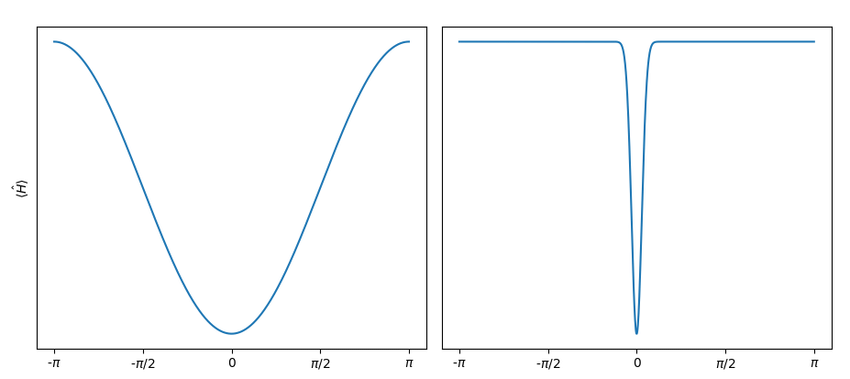
\includegraphics[width=\textwidth]{src/Appendices/example-of-a-barren-plateau.png}
    \caption{
        An illustrative example of a barren plateau and narrow gorge.
        On both plots: the expectation value of a Hamiltonian for a single parameter in the quantum circuit.
        On the left: expectation value landscape in the absence of barren plateau. 
        On the right expectation value landscape in case of a barren plateau.
        Figure from Chen et al. \cite{tillyVariationalQuantumEigensolver2021}.
    }
    \label{fig: Barren Plateau Example}
\end{figure}



This research project undertakes a study that aims to survey and compare some countermeasure approaches to mitigate or avoid the effect of BP in the QNN development under VQA methods. 
The main work of this article is summarized: 
We provide some essential background for VQA and QNN;
We define the BP phenomenon and the causes that would lead to this issue; 
The composition of known methods to address the matter of concern will be introduced, as well as performance comparison to identify the best approach; 
Finally, we conclude the paper with some open issues and prospects for the field.


\input./ProjectDesc/Content/problem}

\subsection{Objectives}
To answer the above research question, it will be necessary to meet the following research objectives:
% \begin{enumerate}
%     \item Provide the background information for quantum computing, VQA and QNN, which enables definition of the research question (completed, see \ref{Sec: Background Section});
%     \item Define the BP problem and the causes that would lead to this phenomenon \cite{wangNoiseinducedBarrenPlateaus2021,zhaoAnalyzingBarrenPlateau2021} (completed, see \ref{Problem Section});
%     \item Investigate several methods to mitigate or avoid BP \cite{pesahAbsenceBarrenPlateaus2021, pattiEntanglementDevisedBarren2021,liuParameterInitializationMethod2021};
%     \item Compare advantages and disadvantages of the identified methods to identify the most appropriate approaches in different circumstances;
%     \item Conclude the research with summary and open issues still remaining for the future research.
% \end{enumerate}
\begin{itemize}
    \item Trimester 1 - 2022: Literature review and research design
          \begin{enumerate}
              \item Provide the background information for quantum computing, VQA and QNN, which enables definition of the research question (completed, see Section \ref{Sec: Background Section});
              \item Define the BP problem and the causes that would lead to this phenomenon \cite{wangNoiseinducedBarrenPlateaus2021,zhaoAnalyzingBarrenPlateau2021} (completed, see Section \ref{Problem Section});
              \item Investigate several methods to mitigate or avoid BP \cite{pesahAbsenceBarrenPlateaus2021, pattiEntanglementDevisedBarren2021,liuParameterInitializationMethod2021} (completed as minimum viable artefact, see Section \ref{Minimum Artefact section});
          \end{enumerate}
    \item Trimester 2 - 2022: Addressing the gaps
          \begin{enumerate}
              \item Investigate several methods to mitigate or avoid BP \cite{pesahAbsenceBarrenPlateaus2021, pattiEntanglementDevisedBarren2021,liuParameterInitializationMethod2021};
              \item Compare advantages and disadvantages of the identified methods to identify the most appropriate approaches in different circumstances;
              \item Conclude the research with summary and open issues still remaining for the future research.
          \end{enumerate}
\end{itemize}

\subsection{Success Criteria}
\begin{enumerate}
    \item Review 3-4 different methods of dealing with BP
    \item What method is the most suitable for different contexts;
    \item Provide guidelines for mitigating BP;
\end{enumerate}



\subsection{Motivation}
There are indeed some problems with QNN training, as pointed out in section \ref{Background Section}, namely the Barren Plateaus phenomenon.
Luckily, some studies addressed the problem: \cite{pesahAbsenceBarrenPlateaus2021,pattiEntanglementDevisedBarren2021,liuParameterInitializationMethod2021}.
We bring together those methods to identify the most suitable for different circumstances.
We also give a reference and guidelines for mitigating or avoiding BP, and therefore, VQAs can solve more practical problems. 
This project provides an approach to Quantum Algorithms for Machine Learning and Computer scientists.

\bibliographystyle{jcabbrv} % Sorted and "note" fields removed
\bibliography{src/References/zoteroReferences.bib}
% 	\thispagestyle{empty}
\begin{titlepage}
    
\includegraphics[width=0.25\textwidth]{src/CoverPage/Deakin_Logo.jpeg}
        \begin{center}
        \vspace*{4cm}
        {\LARGE Investigation of Barren Plateaus in Quantum Neural Network Development}
        \vspace{3cm}
            \begin{large}   
    
        
            \bf Literature Review Draft
            \vspace{1cm}
        
            \bf \today \\
            T1-2022        
        
            \vspace{3cm}
            \textbf{Thanh Nguyen}\\
            STUDENT ID 218583133 \\
            COURSE - Bachelor of IT Honours (S470)
            \vfill

            \bf \normalsize Supervised by: Prof, Jacob Cybulski\\
       
        \end{large}  
   \end{center}
\end{titlepage}


% \tableofcontents
% \pagebreak
\section {Literature Review}

\section{Overview}
This paper reviews the Quantum Neural Networks and Variational Quantum Algorithms, their structures, and the mathematics underneath. 
We aim to explore their gaps in studies, especially the factors that would lead to the problem of Barren Plateaus.
Then, we review and compare some methods to counter minimise the Barren Plateaus phenomenon by addressing those factors.

In general, Barren Plateaus can be noise-induced \cite{wangNoiseinducedBarrenPlateaus2021}, which means that the noise from quantum hardware affects the trainability; 
or circuit-induced \cite{mccleanBarrenPlateausQuantum2018}, as a result of the circuit design and initialisation parameters.
This research focuses on mitigating the effect of circuit induced Barren Plateaus by reviewing some of the available studies \cite{pesahAbsenceBarrenPlateaus2021, cerezoCostFunctionDependent2021, skolikLayerwiseLearningQuantum2021}.
From this point onward, we will address the term 'Noise-Induced Barren Plateaus' as 'Barren plateaus' for simplicity.

We strongly recommend readers to have foundation knowledge in Quantum Computing, Linear Algebra and Machine Learning. 
The 2020 Qiskit course \cite{2020QiskitGlobal} is a good start for beginners, this course provide very basic mathematics, theories and practices. 
The book \cite{sutorDancingQubitsHow2019} by Robert S. is also recommended while taking the 2020 Qiskit course, other than the basics of Quantum Computing, the author presented an overview of the current quantum hardware and simulator

\subsection{VQA and QNN}
\label{VQA}

Hybrid techniques involving quantum circuits and classical optimisers have been proposed to overcome the restrictions of Noisy Intermediate-Scale Quantum (NISQ) \cite{brooksQuantumSupremacyHunt2019} devices.
Those restrictions include inability of NISQ devices to achieve fault-tolerance, restrictions on the number of the available qubits per their quantum processors, and the limited depth of practically executable quantum circuits.
Moreover, quantum circuits and their gates are static by design, which means that input data into a quantum algorithm must be encoded as gates of the circuit implementing this algorithm. This implies that each instance of quantum algorithm use results in a new and distinct quantum circuit. This creates a barrier to using quantum circuits in support of efficient algorithm optimisation and training of quantum machine learning models.

Nevertheless, hybrid techniques, which combine classical and quantum techniques, allow development of \emph{variational circuits} (or circuit templates) with trainable parameters that can be iteratively refined by instantiating their values to create a static circuit using a traditional (classical) computer (i.e. when training VQAs) \cite{cerezo2021variational}, but which can then be efficiently executed on a quantum machine.
In this way, it is also possible to rely on range of classical optimisers, which treat variational circuits as black boxes capable of yielding outputs from inputs and the trainable parameters.

Consider a simple problem that we want to solve using VQA, given access to the training data.
The first step is to construct a \textit{cost function} $C$ used to search for an optimal set of circuit parameters, which is achieved by minimising the cost function during the training process.
We can simplify the development of variational circuits by composing the circuit templates called \textit{ansatze}.
\textit{Ansatz} is the parameterised circuit that depends on a set of parameters $\theta$. We aim to train the ansatze by optimising the parameters $\theta$s so that the cost function $C$ reaches its minimum, thus satisfying:
\begin{equation}
    \theta^* = \underset{\theta}{\arg \min} \;C(\theta)
    \label{optimize theta with ansatz}
\end{equation}

In short, the cost function $C(\theta)$ is calculated using the quantum computer, while the classical optimiser trains the parameters $\theta$. Figure \ref{VQA diagram} explains the VQA architecture and elaborates its training process in more detail.

\begin{figure}
    \centering
    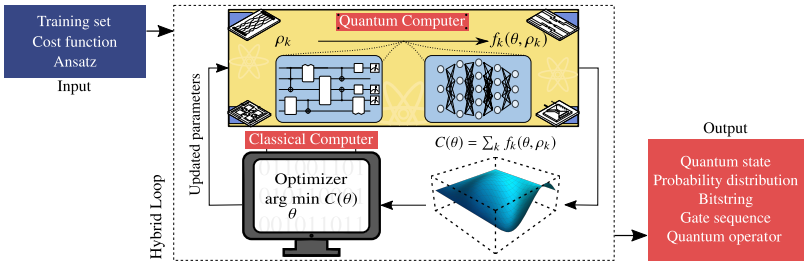
\includegraphics[width=\textwidth]{LiteratureReview/Appendices/vqadiagram.png}
    \caption{
        An illustrative diagram of VQA.
        The algorithm is a hybrid loop that receives:
        A cost function $C(\theta)$ for $\theta$ is a set of parameters that encodes the solution;
        An ansatz that receives trainable parameter $\theta$ to solve the task;
        A set of training data $\{\rho_k\}$.
        We use the quantum computer to calculate the cost for each iteration, then use an optimisation algorithm in a classical computer to find the global minima in the cost landscape $C(\theta)$ and thus satisfy the problem in Eq. (\ref{optimize theta with ansatz}).
        VQA's result is an approximation of the problem solution, which can take forms as in the red box.
        Figure from Cerezo et al. \cite{cerezo2021variational}.
    }
    \label{VQA diagram}
\end{figure}

\subsubsection{The Cost Function}
Encoding the problem into a cost function is the first step in solving a problem using VQA \cite{cerezo2021variational}.
The cost function is equivalent to that used in classical machine learning.
It maps the values of the trainable parameters $\theta$ into real values, which represent the measure of distance from an optimum solution.
For a function $f$ that receives input states $\{\rho_k\}$, observables $\{O_k\}$, and a parameterized circuit $U(\theta)$, the cost is expressed as:
\begin{equation}
    C(\theta) = f(\{\rho_k\}, \{O_k\}, U(\theta)) \;,
\end{equation}
or this form with a set of functions $\{ f_k \}$ and the square of a distance matrix given as its trace $Tr$:
\begin{equation}
    C(\theta) = \sum_k f_k \left(\Tr[ O_k U(\theta) \rho_k U^\dagger(\theta) ]\right) \;,
    \label{Cost function}
\end{equation}

For the function to be used as a cost function it must meet a number of criteria:
(1) The cost function must be 'faithful' and 'operationally meaningful', such that the minimum of $C(\theta)$ should correspond to the solution of the problem, and the lower cost function indicate a better solution in general;
(2) Cost function must be 'efficiently estimable' by the measurement conducted on a quantum computer and the subsequent classical post-processing;
(3) The cost must be 'trainable', such that the parameters $\theta$ could be efficiently optimised.

\subsubsection{Ansatze}
\begin{figure}
    \centerline{
    \Qcircuit @C=1em @R=0em {
    & \multigate{2}{U_1(\theta_1)}    & \multigate{2}{U_2(\theta_2)}    & \qw &        & & \multigate{2}{U_L(\theta_L)}   & \qw\\
    & \ghost{U_1(\theta_1)}           & \ghost{U_2(\theta_2)}           & \qw & \cdots & & \ghost{U_L(\theta_L)}          & \qw\\
    & \ghost{U_1(\theta_1)}           & \ghost{U_2(\theta_2)}           & \qw &        & & \ghost{U_L(\theta_L)}          & \qw
    \gategroup{1}{2}{3}{7}{.6em}{--}
    }
    }
    \centerline{$U(\theta)$}
    \centerline{}
    \centerline{}
    \centerline{
    \Qcircuit @C=1em @R=0em{
    & \multigate{1}{}   & \ctrl{2}  & \gate{}           & \qw \\
    & \ghost{}          & \qw       & \multigate{1}{}   & \qw \\
    & \gate{}           & \targ     & \ghost{}          & \qw
    \gategroup{1}{2}{3}{4}{.6em}{--}
    }
    }
    \centerline{$U_l(\theta_l)$}
    \caption{
        A diagram of a sample ansatz (above), the ansatz is a sequence of unitaries $U_l(\theta_l)$ (below).
        The unitary $U(\theta)$ receives parameters $\theta$ is expressed by $L$ layers of unitaries $U_l(\theta_l)$ for $l$ is the layer indices.
        Each $U_l(\theta_l)$ is a circuit composed of a mix of parameterised and unparametrised gates.
    }\label{Ansatz diagram}
\end{figure}

In physics and mathematics, \emph{ansatz} (plural \emph{ansatze}) is an educated guess or a starting point from which you start looking for a solution to the problem at hand. In quantum computing, \emph{ansatz} is a parameterised circuit, formed as a sequence of unitary (or "atomic") circuits, which is used as a framework for the circuit optimisation.
In general, the location of parameters $\theta$ is determined by the ansatz form and can be trained to minimise the cost.
The ansatz structure can be defined based on the problem (called 'problem-inspired ansatze') or a generic structure (called 'problem agnostic ansatze') that can be used without any relevant information available \cite{cerezo2021variational}.

The cost function in Eq. (\ref{Cost function}) encodes the parameters $\theta$ in a unitary $U(\theta)$ and applies to the input states of the circuit.
The figure \ref{Ansatz diagram} shows that $U(\theta)$ can be expressed as a product of $L$ consecutive unitaries:
\begin{equation}
    U(\theta) = U_L(\theta_L) \cdots U_2(\theta_2) U_1(\theta_1)\;,
\end{equation}
with each layer:
\begin{equation}
    U_l(\theta_l) = \prod_m e^{-i\theta_m H_m} W_m
\end{equation}
for unparamaterized unitary $W_m$, hermitian operator $H_m$, and $\theta_l$ is the $l$-th element of $\theta$.

\subsubsection{Gradients}
After defining the cost function and a suitable ansatz, we train the parameter $\theta = \{\theta_{l}\}$ to solve the problem in Eq. (\ref{optimize theta with ansatz}) \cite{cerezo2021variational}.
The cost function gradient helps the optimiser to find the global minima.
Consider the cost function in Eq. (\ref{Cost function}), for a unitary that parameterises rotation $e^{i \theta_l \sigma_{l}}$, where $\theta_l$ be the $l$-th element of $\theta$, $\sigma_l$ is a Pauli rotation operator.
We can evaluate the gradient with the parameter-shift rule:
\begin{equation}
    \frac{\partial C}{\partial\theta_l}
    = \sum_k \frac{1}{2 \sin{\alpha}}
    \left(
    \Tr[O_k U^\dagger(\theta_+) \rho_k U(\theta_+)]
    - \Tr[O_k U^\dagger(\theta_-) \rho_k U(\theta_-)]
    \right) \;,
    \label{Parameter-shift rules}
\end{equation}
with $\theta_{\pm} = \theta \pm \alpha e_l$, $\alpha \in \mathbb{R}$ and $e_l$ is a vector such that its $l$-th position have the value of 1, or else 0.

Essentially, we can shift the $l$-th parameter by some amount $\alpha$, and Eq. (\ref{Parameter-shift rules}) will calculate the gradient.


\subsubsection{Optimisers}
The accuracy of VQA greatly depends on the optimisation method.
Typically, we can achieve the solution by making successive moves along the gradient direction.
This optimisation approach is within the scope of stochastic gradient descent (SGD).
One example of SGD is the ADAM optimiser \cite{kingmaAdamMethodStochastic2014}, which can vary the size of the steps taken during optimisation to produce more efficient and precise results compared to the basic SGD.


\subsubsection{About QNN}
VQA is also the most widely used method for developing Quantum Neural Network (QNN) circuits.
As a result, QNN inevitably inherited some of VQA's features and flaws.
Many quantum machine learning models suffer from the issue of \textit{barren plateaus} \cite{zhaoReviewQuantumNeural2021} that prevent the growth of circuit depth and lead the training of parameters to a dead end.
When training a QNN framework with a large number of qubits, this phenomenon is likely to occur; the objective function becomes flat, whereby its gradient is nearly zero across a large plateau, making it nearly impossible to identify the global minimum (also defined by the zero gradient), \cite{mccleanBarrenPlateausQuantum2018, zhaoAnalyzingBarrenPlateau2021} causing inefficiency in circuit training.
We will discuss this matter in later sections.

% Some architectures of QNN have been proposed to counter this problems, for example: 
% Quantum Tensor Neural Network (QTNN) \cite{hugginsQuantumMachineLearning2019} which achieved a balance of computational efficiency and expressive power. 
% The tensor network can reduce the required number of qubits to process high-dimensional data with powerful optimisation algorithms.
% An alternative solution is to rely on Quantum Recurrent Neural Network (QRNN) which is constructed as a parameterised circuit \cite{takakiLearningTemporalData2021}, with some qubits being initialised and measured at each step while others memorise the past data.

Many types of QNN models also suffer from the emergence of barren plateaus during their training (although for different reasons), for example in:
Quantum Boltzmann Machines \cite{shinguBoltzmannMachineLearning2021, zoufalVariationalQuantumBoltzmann2021},
Quantum Perceptrons \cite{kristensenArtificialSpikingQuantum2021} and
Quantum Generative Adversarial Networks \cite{dallaire-demersQuantumGenerativeAdversarial2018, lloydQuantumGenerativeAdversarial2018}.
It is worth noting that Quantum Convolutional Neural Networks (QCNNs) do not exhibit barren plateaus \cite{pesahAbsenceBarrenPlateaus2021}.
Thus, training convergence is more successful for QCNNs under random initialisation.

Studies have shown that Neural Network training and execution performance involving quantum machines can be significantly higher than that achievable using today's classical hardware \cite{abbasPowerQuantumNeural2021, colesSeekingQuantumAdvantage2021}. Consequently quantum neural nets may find some promising applications, for example, in breast cancer prediction \cite{liModelAlgorithmQuantuminspired2014} or image processing \cite{matsuiQubitNeuralNetwork2009}.

\subsection{Barren Plateaus, Gradients, Trainability Issue} \label{Barren Plateaus section}

When training a quantum circuit, three important elements are needed to construct the initial variational circuit and a cost function: some reference states (the inputs), a parameterised unitary operation (the circuit, or ansatz), and an observable $O$ (the outputs). Then we also need to select a suitable classical optimiser.

The next step is to evolve this variational circuit from the initially random state of circuit parameters to the circuit instantiated with the optimal parameter values.

The process is iterative. At each cycle of the optimisation, the optimiser suggests the values for the variational circuit parameters, optionally increases the circuit depth, instantiates the circuit with the parameters values, and runs thus created executable circuit on a quantum machine.
The obtained outputs can subsequently be compared with the observables and the current value of the cost function calculated, so that the optimisation routine could then suggests the new set of parameters for the evolving circuit \cite{cerezo2021variational}.
By changing the circuit parameters, we are exploring an optimisation landscape to find a global minimum for the cost function, and thus the optimum circuit parameters.
The properties of this landscape heavily depend on the structure of the parameterised circuit (derived from input-output pairs and the selected ansatz) and the selected cost function.

Typically, two starting ingredients for problem-solving using heuristic ansatzes are a randomly parameterized circuit $U$ and a set of random initialization parameters $\vec{\theta}$, non-parameterized unit $W_l$ for each layer $l$ \cite{mccleanBarrenPlateausQuantum2018}:
\begin{equation}\label{Parameterized Circuit}
    U(\vec{\theta})
    = U(\theta_1, \cdots, \theta_L)
    = \prod_{l=1}^L U_l(\theta_l)W_l
\end{equation}
With $L$ is the depth of the circuit. Consider a cost function $C(\theta)$ with an observable $O$ and the ansatz $U$:
\begin{equation}
    C(\vec{\theta})
    = \bra{0} U(\vec{\theta})^\dagger OU(\vec{\theta}) \ket{0}
\end{equation}

The gradients are the derivatives of the cost function respectively to the parameters and have a severe impact on the performance of the training model:
\begin{equation}
    \partial_l C = \frac{\partial C(\vec{\theta})}{\partial\theta_l}
\end{equation}
McClean et al. \cite{mccleanBarrenPlateausQuantum2018} also pointed out that whenever the random parameterised circuits reach the depth $O(n^{1/L})$ on a $L$-dimensional array, the gradient of the cost function will vanish.
The variance of the gradient shrinks exponentially with the number of qubits $n$:
\begin{align}
    \langle \partial_k C\rangle & = 0  \label{Vanish Gradient}                  \\
    \mathrm{Var}[\partial_k C]  & \approx 2^{-n}  \label{Variance expo smaller}
\end{align}
Barren plateaus is a serious issue for circuit optimisation because the flatter the landscape is, the more challenging it is to search for the location of the global cost minimum.
Compared to the gradient in a deep classical network which vanishes exponentially in the number of layers, for the QNN case, the gradient grows exponentially small with the number of qubits \cite{mccleanBarrenPlateausQuantum2018}.

Additionally, the choice of the initiate parameter $\theta$ is also an important factor. When an ansatz is randomly initialised, the algorithm may start far from the solution, at a local minimum, or even on the surface of a barren plateau.

To summarise, the following factors can lead to barren plateaus in QNN and VQA:
\begin{itemize}
    \item \textbf{\emph{The ansatz depth and the number of qubits}}
    \item \textbf{\emph{Random initialization parameters}}
\end{itemize}



\subsection{Addressing Parameterized circuit depth}
\subsubsection{Shallow Circuits, Local Cost Function}
\begin{figure} 
    \centerline{
        \Qcircuit @C=1em @R=0em {
        & \multigate{4}{U(\theta)}    & \meter\\
        & \ghost{U(\theta)}           & \meter\\
        & \ghost{U(\theta)}           & \meter\\
        & \ghost{U(\theta)}           & \meter\\
        & \ghost{U(\theta)}           & \meter\\
        }
    }
    \centerline{a) Global Cost Function}
    \centerline{
        \Qcircuit @C=1em @R=0em {
        & \multigate{4}{U(\theta)}    & \meter\\
        & \ghost{U(\theta)}           & \qw\\
        & \ghost{U(\theta)}           & \qw\\
        & \ghost{U(\theta)}           & \qw\\
        & \ghost{U(\theta)}           & \qw\\
        }
    }
    \centerline{b) Local Cost Function}
    \caption{
        Global Cost Function and Local Cost Function.
        a) Global Cost Function compares the states in exponentially large Hilbert space.
        b) Local Cost Function compares the states at single qubit level.
    }\label{cost functions}
\end{figure}

Cerezo et al. has demonstrated \cite{cerezoCostFunctionDependent2021} properties of a 'local cost function' in a parameterised circuit. 
Let us recall the cost function $C$ with an operator $O$, the ansatz $U(\theta)$ and some input states $\rho$:
\begin{equation}
    C = \Tr\left[
    OU(\theta) \rho U^\dagger(\theta)
    \right],
\end{equation}
the authors called this cost function as 'Global Cost Function' $C_G$, which can inhabit Barren Plateaus. Compared to the proposed 'Local Cost Function':
\begin{equation}
    C_L = \Tr\left[
    O_L U(\theta) \rho U^\dagger(\theta)
    \right],
\end{equation}
with
\begin{equation}
    O_L = I- \frac{1}{n} \sum^n_{j=1}\rho_j \bigotimes I_{\overline{j}},
\end{equation}
where $I_{\overline{j}}$ is the identity on all qubits except the qubit in $j$-th position.



if a \almarginpar{Explain what is "local" vs "global" cost function}\underline{local cost} function is used, then there is a lower bound for the variants of the gradients that depends on the number of qubits and some configurations of the circuit. 
For a $L$-layered ansatz, let the variance $\mathrm{Var}[\partial_v C]$ of the partial derivative of the cost function $C$, the lower bound $G_n$ for the variance is:
\begin{equation}
    G_n(L,l) \leq \mathrm{Var}[\partial_k C]
\end{equation}
\begin{equation}
    G_n(L,l) = \frac{{2}^{m(l+1)-1}}{{({2}^{2m}-1)}^{2}{({2}^{m}+1)}^{L+l}}
    \times \mathop{\sum}\limits_{i\in {i}_{{\mathcal{L}}}}\mathop{\sum}\limits _{{(k,k^{\prime} )\in {k}_{{{\mathcal{L}}}_{\text{B}}}}\atop {k^{\prime} \geqslant k}}{c}_{i}^{2}\epsilon ({\rho }_{k,k^{\prime} })\epsilon ({\widehat{O}}_{i})\ ,
\end{equation}
Where the forward light-cone $\mathcal{L}$ is a set of gates with at least one input connected to the output of a block $W$; 
The backward light-cone $\mathcal{L}_\text{B}$ is a set of gates with at least one output connected to the input of block $W$;
$S_k$ is the $m$-qubit subsystem;
$i_{\mathcal{L}}$ is a set of indices such that the operators $\hat{O_i}$ act on qubits in $\mathcal{L}$;
$k_{\mathcal{L}_B}$ is a set of indices such that the subsystem $S_k$;

\almarginpar{What is $G_n$}If the total depth $L$ is in the range $O(\log(n))$ of the number of qubits (a shallow configuration), then the lower bound cannot vanish faster than $\Omega(1/\mathrm{poly}(n))$. 
Thus, no Barren Plateau occurs in this case.\almarginpar{You throw lots of formulas in but do not explain much}



\subsubsection{Layerwise learning for quantum neural networks}

There is another method that manipulates the circuit depth throughout the training period studied by Skolik et al. \cite{skolikLayerwiseLearningQuantum2021}. 
In more detail, the algorithm consists of two phases:

\almarginpar{Good find "qcircuit"!}\textbf{The first phase} constructs the ansatz by adding layers one by one, with the parameters are all initially zero. For a small number $s$ of starting layers, the set of parameters $\vec{\theta_1}$, and $W$ operators connecting qubits, then the initial layers $l_1(\vec{\theta_1})$ is presented:

\begin{equation}
    l_1(\vec{\theta_1})
    = \prod_{j=1}^s U_{1_j}(\vec{\theta_{1_j}}) W \;,
\end{equation}

Where each consecutive layer $l_i(\vec{\theta_i})$ of form
\begin{equation}
    l_i(\vec{\theta_i})
    =U_i(\vec{\theta_i}) W \;,
\end{equation}
is added after a certain number of epochs and the previous layers' parameters become fixed. 
One epoch is the set of iterations for the algorithm to see each training sample; an update of all trainable parameters is called one iteration.

This process can stop when a certain circuit depth is reached or until the objective function's value does not improve with additional layers.
Figure \ref{ll circuit} provides an illustrative example of the final circuit.
Eventually, we obtain the final circuit of $L$ layers:

\begin{equation}
    U(\vec{\theta})
    = \prod_{i=0}^L l_i (\vec{\theta_i}) \;.
\end{equation}
\begin{figure} 
    \centerline{
        \Qcircuit @C=1em @R=0em {
        & \multigate{4}{l_1(\vec{\theta_1})}    & \multigate{4}{l_2(\vec{\theta_2})}    & \qw &        & & \multigate{4}{l_i(\vec{\theta_i})}   & \qw\\
        & \ghost{l_1(\vec{\theta_1})}           & \ghost{l_2(\vec{\theta_2})}           & \qw &        & & \ghost{l_i(\vec{\theta_i})}          & \qw\\
        & \ghost{l_1(\vec{\theta_1})}           & \ghost{l_2(\vec{\theta_2})}           & \qw & \cdots & & \ghost{l_i(\vec{\theta_i})}          & \qw\\
        & \ghost{l_1(\vec{\theta_1})}           & \ghost{l_2(\vec{\theta_2})}           & \qw &        & & \ghost{l_i(\vec{\theta_i})}          & \qw\\
        & \ghost{l_1(\vec{\theta_1})}           & \ghost{l_2(\vec{\theta_2})}           & \qw &        & & \ghost{l_i(\vec{\theta_i})}          & \qw\\
        }
    }
    \caption{
        Constructing the ansatz from shallow layers.
    }\label{ll circuit}
\end{figure}


\textbf{The second phase} takes the pre-trained circuit from phase one and trains \almarginpar{What are these?}\underline{larger adjacent partitions} of layers at a time. 

\subsection{Addressing Random initialization parameters}

\subsubsection{Layerwise learning for quantum neural networks \texorpdfstring{\cite{skolikLayerwiseLearningQuantum2021}}{}}
The algorithm in \cite{skolikLayerwiseLearningQuantum2021} starts with training a shallow circuit to its best, then extends the circuit and uses the best parameter achieved in the previous step for the newly extended circuit. 
Note that only the new parameters are allowed to vary while the previous parameters are frozen.
Thus, the randomness is contained to only shallow sub-circuits in phase one during the whole routine and minimizes the probability of meeting a plateau during the process.


\subsubsection{An initialization strategy for addressing Barren Plateaus in parameterized quantum circuit \texorpdfstring{\cite{grantInitializationStrategyAddressing2019}}{}  }

Grant et al. have addressed the Random initialization parameter so that the early training steps do not start on a plateau region. 
The idea is to divide the big parameterized circuit into blocks and initialize each block so that the result is a fixed unitary matrix, i.e., an identity operation. 
The method is as follows: partition the circuit into $M$ blocks of depth $L$; for each block, initiate some parameters with random values, and fix the remaining parameters in a way that results in a fixed unitary matrix, i.e., invert the first part so that each block implements an identity operation.

The depth $L$ is chosen to be shallow enough so that each block cannot reach 2-designs. For any $m = 1, \cdots, M$, the parameters $\theta$, the block is presented as:
\begin{equation}
    U_m(\theta_m)
    = \prod_{l=L}^1 U_l(\theta_{l,1}^m) \prod_{l=1}^L U_l(\theta_{l,2}^m).
\end{equation}
The starting parameter $\theta_{l,1}$ can be chosen randomly, while the values for $\theta_{l,2}$ are chosen such that $U_l(\theta_{l,2}) = U_l(\theta_{l,1})^\dagger$:
\begin{equation}
    U_m(\theta_m)
    = \prod_{l=L}^1 U_l(\theta_{l,1}^m)
    \prod_{l=1}^L U_l(\theta_{l,1}^m)^\dagger
    = I_m,
\end{equation}
resulting identity blocks for the circuit:
\begin{equation}
    U(\theta^{init})
    = \prod_{m=M}^1 U_m(\theta_m)
    = \prod_{m=M}^1 I_m
    = I.
\end{equation}

\subsection{Comparison and Discussion}
We will now discuss the main characteristics, the pros and cons of each of the previously discussed methods of dealing with barren plateaus while training VQAs and QNNs in particular.
As has been established above, the main causes of the barren plateaus phenomenon include: the excessive circuit depth, the large number of qubits in use and poorly initialised circuit parameters.
Consequently, we will identify characteristics of each method based on how they address these factors.
Table \ref{quick comparison of methods} provides the methods comparison in a concise form.

There are two distinct approaches in dealing with the ansatz depth, either setting the bounds \cite{cerezoCostFunctionDependent2021} or allowing unlimited depth \cite{skolikLayerwiseLearningQuantum2021, grantInitializationStrategyAddressing2019}.
The first approach is studied by Cerezo et al. \cite{cerezoCostFunctionDependent2021}.
The authors discovered that the gradient vanishes at different rate depends on the circuit depth, so they define the bounds on the circuit depth such that the cost function landscape can maintain its slope.
We have two implementations of the second approach, they both have the unlimited ansatz depth but different in the construction procedure.
Skolik et al. \cite{skolikLayerwiseLearningQuantum2021} construct the ansatz by adding consecutive layers until there is no improvement in training efficiency.
On the other hand, Grant et al. \cite{grantInitializationStrategyAddressing2019} train the circuit without altering any properties of the ansatz.

There are two techniques to dealing with cost function.
The global cost function compares the states of all qubits used in the ansatz, this cost function is widely used in QNN development.
Skolik et al. and Grant et al. also adopted this cost function in their studies.
The local cost function compares the states of some qubits used in the ansatz, this cost function is studied by Cerezo et al. \cite{cerezoCostFunctionDependent2021} in combination with the depth-bounded ansatz.

The initial parameters can be either randomised, or predefined.
As the gradient is calculated with those parameters, randomised parameters can land into a barren plateaus.
However this is not the case in the study of Cerezo et al. which completely eliminate the near-zero gradient phenomenon.
Since the plateau does not exist and the gradient can maintain its slope, the randomised initial parameter is a viable option.
For the case of predefined initial parameters, we have two studies.
Skolik et al. \cite{skolikLayerwiseLearningQuantum2021} proposed an algorithm that starts with zeros parameters in a small ansatz.
Their algorithm allows the parameters to be trained as the ansatz grow over time.
Grant et al. \cite{grantInitializationStrategyAddressing2019} divide the ansatz into shallow blocks and configure the parameters such that each block implement an identity operation.
The authors aimed to avoid non-zero gradients in the first training iteration, which guaranteed the initialisation away from a barren plateau and allowed the circuit to be trained efficiently.
However, this method cannot ensure the algorithm will not go into a barren plateau again in further iterations of optimization algorithm.
Overall, the authors manipulated the starting parameters to achieve trainability, but the risk of going to a plateau is still there.

Finally, it is worth mentioning that Quantum Convolutional Neural Networks (QCNNs) and QNNs with tensor network architectures do not have Barren Plateaus \cite{congQuantumConvolutionalNeural2019}.

\begin{table}[]
    \centering
    \begin{tabular}{|p{3cm}|p{2cm}|p{2cm}|p{2cm}|p{2cm}|}
        \hline
        \textbf{Method /\newline Aspect}             & \textbf{Local cost function, shallow circuits} & \textbf{Identity Blocks} & \textbf{Layerwise learning} & \textbf{QCNN} \\
        \hline \hline
        \raggedright\emph{Ansatz depth}              & Bounded                                        & Any length               & Any length                  & Any length    \\
        \hline
        \raggedright\emph{Qubits to be measured}     & Limited                                        & All qubits               & All qubits                  & All qubits    \\
        \hline
        \raggedright\emph{Initial Parameters}        & Randomised                                     & Restricted               & Restricted                  & Randomised    \\
        \hline \hline
        \raggedright\emph{Effect to Barren Plateaus} & Eliminated                                     & Avoided                  & Avoided                     & Eliminated    \\
        \hline
    \end{tabular}
    \caption{A compact comparison of the reviewed methods.}
    \label{quick comparison of methods}
\end{table}


\subsection{Conclusion}
In this literature review, we went through the definition of QNN and VQA to point out the challenging Barren Plateaus phenomenon. 
Some studies have attempted to address this issue, but the problem has not been entirely resolved.
We have selected three methods directly related to the main factors that lead to this phenomenon: the initialization process the circuit depth and the number of qubits.
Finally, we compactly discuss the three methods by comparing their properties, pros and cons.
This literature review also suggests that an empirical study is required to identify the best strategies for particular situations.
%     \section{Research Design} \label{Research Design section}
In this section, we design an experimental methodology to rigorously explore the range of possible approaches to dealing with barren plateaus in QNN/VQA development, thus answering the study research question (see Section \ref{Problem Section}).

% \thispagestyle{empty}
\begin{titlepage}
    
\includegraphics[width=0.25\textwidth]{src/CoverPage/Deakin_Logo.jpeg}
        \begin{center}
        \vspace*{4cm}
        {\LARGE Investigation of Barren Plateaus in Quantum Neural Network Development}
        \vspace{3cm}
            \begin{large}   
    
        
            \bf Research Design Draft
            \vspace{1cm}
        
            \bf \today \\
            T1-2022        
        
            \vspace{3cm}
            \textbf{Thanh Nguyen}\\
            STUDENT ID 218583133 \\
            COURSE - Bachelor of IT Honours (S470)
            \vfill

            \bf \normalsize Supervised by: Prof, Jacob Cybulski\\
       
        \end{large}  
   \end{center}
\end{titlepage}


% Duplicated
% \subsection{Research Question and Motivation}
For this research project, we are interested in the problem "How to mitigate or avoid Barren Plateaus (BP) in the QNN development in the VQA circuit construction approach."

There are indeed some problems with QNN training, as pointed out in Project Description and Literature review, namely the Barren Plateaus phenomenon.
Luckily, some studies have addressed the problem: \cite{pesahAbsenceBarrenPlateaus2021,pattiEntanglementDevisedBarren2021,liuParameterInitializationMethod2021}.
We bring together those methods to identify the most suitable for different circumstances.
We also give a reference and guidelines for mitigating or avoiding BP, and therefore, VQAs can solve more practical problems.
 

\subsection{Research Context}

As explained in the previous section (Section \ref{Literature Review section}), the VQA approach to circuit design for QNN construction overcomes many constraints of static quantum circuits. Most importantly, it allows the construction of trainable circuits, which support the development of practical applications in optimisation and machine learning.
However, we have observed the existence of barren plateaus, causing the variance of the cost function gradient to vanish exponentially with the number of qubits.
We have thus investigated three methods to mitigate this phenomenon, i.e. by using a local cost function with shallow circuits, by relying on the identity block and by utilising layerwise learning \cite{cerezoCostFunctionDependent2021, liuParameterInitializationMethod2021, skolikLayerwiseLearningQuantum2021}.

In the following sections, we will describe an approach to evaluating these three methods, and at the same time outline an approach to answering the study research question (see Section \ref{Problem Section}). This will be done by conducting a series of experiments such that different methods could be applied to the object of this study. 
This process is known as \emph{technology-oriented empirical research} \cite[sect 2.4]{wohlinExperimentationSoftwareEngineering2012}.

We summarise the adopted research process in Figure \ref{Research Activities Figure}.
Our main objects and the different technical treatments for the experiment are discussed in section \ref{Objects section}, the two phases of the experiment in section \ref{Research Activities section}, and finally the confirmation of results from the experiment in section \ref{Data Collecting Section}.

\begin{figure}
    \centering
    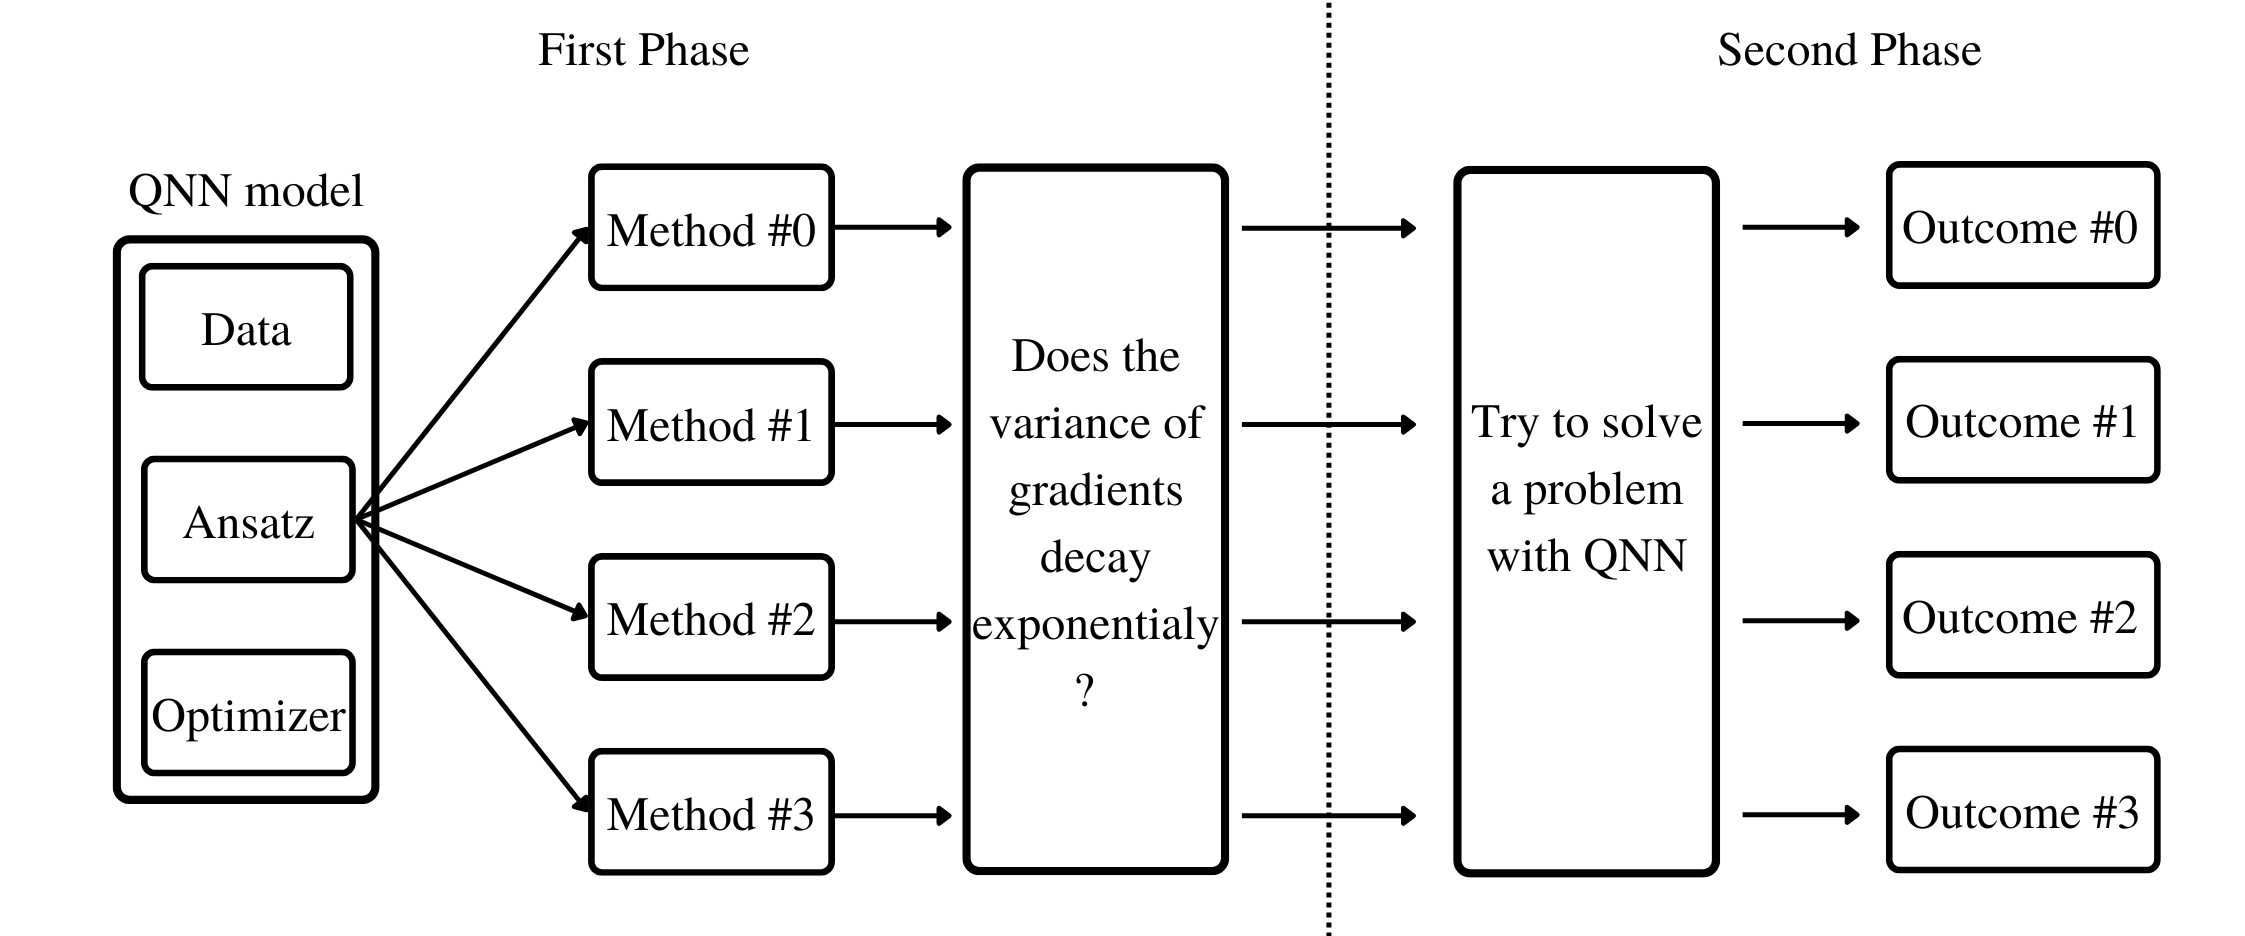
\includegraphics[width=\textwidth]{./ResearchDesign/Appendices/ExperimentDiagram.png}
    \caption{
        The adopted research process.
    }
    \label{Research Activities Figure}
\end{figure}


\subsection{Objects and Parameters}\label{Objects section}
According to the research design guidelines by Wohlin et al. \cite{wohlinExperimentationSoftwareEngineering2012}, we will need to identify the experiment object and the parameters.
While the object is the main entity studied in the experiment, the parameters are the treatments applied to the object.
One advantage of the empirical experiment is that we can have total control of the experiment environment.
As per the literature review (see Section \ref{Literature Review section}), we have identified the object of study is the QNN model.
The parameters that we can apply to the object are:
\begin{itemize}
    \item \textbf{The ansatz choice.} Qiskit framework offers a wide range of ansatz. Refer to the circuit library in Section \ref{Resources section};
    \item \textbf{The ansatz configuration.} The ansatz object from Qiskit is mutable, which means we can configure their properties to fit the experiment activities. For example, the number of qubits, repetition of layers, and initial parameters.
    \item \textbf{The cost function operator.} We can implement a measurement operation at the end of the parameterised quantum circuit to act as the output of the cost function. We discussed two styles of cost functions in Section \ref{Shallow Circuits, Local Cost Function section};
    \item \textbf{The method to mitigate barren plateaus.} We have reviewed three methods in Section \ref{Literature Review section}, and each of them configuresd or trains the ansatz differently (see Table \ref{quick comparison of methods}). Note that QCNN is out of the scope of our experiment. We further describe a \emph{Method 0} such that there are no restrictions in ansatz depth, qubits, cost function, or initial parameters (see Figure \ref{Research Activities Figure} and Table \ref{implementation of methods table}).
\end{itemize}

\subsection{Research Activities} \label{Research Activities section}
According to the exploratory experiment guidelines \cite{oivoSoftwareEngineeringResearch2004}, we apply different treatments to the same object.
We implement the process with an experiment of two phases:

\textbf{In the first phase, we reproduce the barren plateaus phenomenon.}
We use Qiskit \cite{Qiskit} to construct the ansatzes.
For each ansatz, we implement and apply four different methods (see Figure \ref{Research Activities Figure} and Table \ref{implementation of methods table}).
Further implementation of the four methods are discussed in Section \ref{Sec: Treatments for ansatzes}.
By definition of barren plateau as discussed in Section \ref{Sec: Literature Review}, we would expect the shrinking rate of the variance values to be \textit{exponential} (see Figure \ref{Variance Shrinking demo}) if the initial parameter has landed in a barren plateau.
We keep track of the variance and the number of qubits to see if the variance is shrinking at this rate.
The result of the first phase is to determine which combinations of the ansatz and the BP treatment result in the shrinking rate of the loss function gradients.

\textbf{In the second phase, we implement the QNNs and measure their performances}.
With the ansatzes developed from the first step, we can implement the QNN models to test their performances.
The QNN models will be trained with standard data sets provided by Qiskit (refer to Section \ref{Resources section}).

The results of the research activities are discussed in the Subsection \ref{Data Collecting Section}.

\begin{table*}[]
    \centering
    \begin{tabular}{||p{3cm} p{2cm} p{2cm} p{2cm} p{2cm}||}
        \hline
        \textbf{Method /\newline Aspect}      & \textbf{\#0:\newline No restrictions} & \textbf{\#1:\newline Local cost function, shallow circuits} & \textbf{\#2:\newline Identity Blocks} & \textbf{\#3:\newline Layerwise learning} \\
        \hline \hline
        \raggedright\emph{Ansatz depth}       & Any length                            & Bounded                                                     & Any length                            & Any length                               \\
        \raggedright\emph{Cost Function}      & Global                                & Limited                                                     & All qubits                            & All qubits                               \\
        \raggedright\emph{Initial Parameters} & Randomised                            & Randomised                                                  & Restricted                            & Restricted                               \\
        \hline
    \end{tabular}
    \caption{
        A comparison of different methods that applied to the ansatz in phase 1.
        The method $\#$0 is widely applied in construction of QNN ansatzes.
        The other three methods are discussed in Section \ref{Sec: Literature Review}.
    }
    \label{implementation of methods table}
\end{table*}


\begin{figure}
    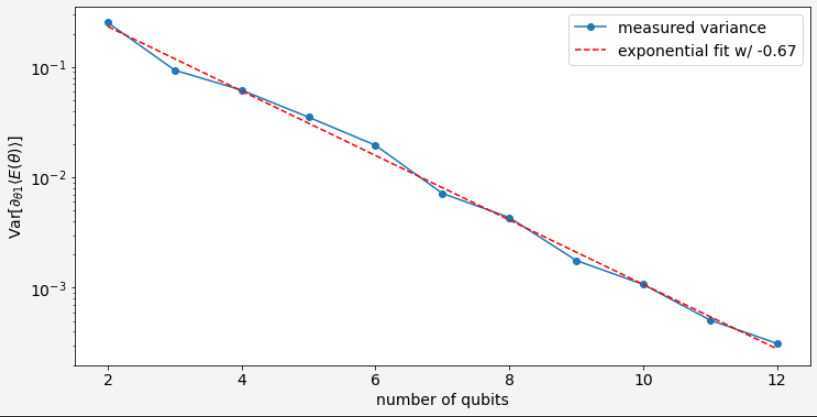
\includegraphics[width=\linewidth]{./ResearchDesign/Appendices/VarianceShrinking.png}
    \caption{
        An example of the barren plateaus phenomenon occurs in a QNN model.
        The variance of the gradient shrinks \textit{exponentially} with the number of qubits.
        Barren plateaus phenomenon prevents optimisation algorithms from navigating the cost function landscape efficiently.
    }
    \label{Variance Shrinking demo}
\end{figure}

\subsection{Criteria}
\label{Criteria section}
We can compare the data of each outcome in from Section \ref{Research Activities section} with these criteria:
\begin{itemize}
    \item Does the model encounter barren plateaus for a large number of qubits?
    \item The quality of the solution;
    \item Loss values per iteration;
    \item The size of the circuit (circuit depth);
    \item The size of the qubit registry (circuit width);
    \item The time required to execute the circuit.
\end{itemize}

\section{Resources}

Most of our resources are open-sources

\begin{itemize}
    \item Python 3.6+: \url{https://www.python.org/downloads/}
    \item Anaconda: \url{https://www.anaconda.com/products/distribution}
    \item Jupyter Notebook: \url{https://jupyter.org/}
    \item Qiskit: \url{https://qiskit.org/}
\end{itemize}

Setup guidelines for Qiskit: 
\url{https://qiskit.org/documentation/getting_started.html}

\subsection{Data Collecting Method and Artefacts Development}
\label{Data Collecting Section}
Here we discuss our method of collecting data from a series of experiments.
We implement the artefact as a Python Notebook that includes all experiment activities and results.
The notebook will require some pre-installed resources to execute (refer to Section \ref{Resources section} for further detail).
As we are conducting experiments on quantum circuits, quantum hardware is also required.
The notebook will be configured to communicate with an IBM quantum device.

% I tried to describe the output form of the python notebook, but it is more like a duplicate with section Research Activities above, so I removed this section
% \almarginpar{I do not understand this}After the first phase, we will obtain the selected ansatzes objects with the four treatments applied (see Figure \ref{Research Activities Figure}) and their variance shrinking rates.
% The shrinking rate can be recorded as a list of numbers and presented as line graphs (for example, see Figure \ref{Variance Shrinking demo}).
% With this data, we can fulfil the first criteria in the Section \ref{Criteria section} by comparing the shrinking rate of each method.

% For the second phase, we will need to further develop the ansatzes from phase one into QNN models. We use the same input data and the optimiser across all models to preserve clarity.
% We run the models along with a benchmark script that records the progress and properties of models (refer to Section \ref{Criteria section})

% Finally, we summarise the research results and present the findings.

\subsubsection{Success Condition}
The experiment will be concluded when these conditions are met:
\begin{itemize}
    \item We have ansatzes that can produce barren plateaus;
    \item The methods are implemented as Python scripts and ready for demonstration;
    \item The ansatzes are implemented as QNN models to solve problems.
    \item The outcomes are evaluated against the criteria.
\end{itemize}

% \subsection{Minimum Artefact and Future Works}
\label{Minimum Artefacts}

The success conditions of the experiment, as discussed, contains the QNN models, the three implementations, the data generated and a guideline to identify which methods to be used on different occasion.
However, the time for the experiment of the unit is limited to one week. We can deliver a minimum viable artefact as a single Python notebook that:
\begin{itemize}
    \item Constructs a QNN using the selected ansatzes that are capable of generating Barren Plateaus;
    \item Implements one out of three methods of dealing with Barren Plateaus as discussed in the literature review;
    \item Verifies the existence of Barren Plateaus for each method above by calculating the variances of their gradients.
\end{itemize}

This artefact outcome will not answer the research question completely.
However, it covers the first half of the experiment and ensures that the outcome is ready to advance to the next steps.

In the later iterations for the experiment, we plan to complete these objectives:
\begin{itemize}
    \item Implement the rest of the three methods;
    \item Verify the trainability of each methods by solving a problem;
    \item Record and plot the \textit{loss value per iteration} and \textit{loss landscape} for each method.
\end{itemize}

To solve a problem with machine learning algorithm, we encode the solution as the \textit{global minimum}, and the gradients of the training model must converge to that minimum point.
Local minimum or Barren Plateaus are the problem that prevent the machine learning model must avoid.
We know the Barren Plateaus is avoided when the variance of the gradient can sustain for a large number of qubit.
However, high variance values does not mean we are in the right direction, the training model can still stuck in a local minimum, which is not the optimal solution.
To verify the trainability of the three methods, we also take this matter into the concern.
Lastly, the final result of these objectives will give confirmation to the hypotheses, as well as answer the research question.

%     \section{Artefact Development Report}
\label{Minimum Artefact section}
\todo{Change this section to include T2 works}
In this section, we describe the progress on the artefact development, the detail and context for the experiments are given as Section \ref{Research Design section}.
We address the process (see Section \ref{Research Activities section}) by implementing a series of exploratory experiments.
The minimum viable artefact is a Python notebook file containing Python scripts to run the experiment.
We run the notebook with IBM Quantum Experience, as it provides online services for running and simulating quantum hardware.
We use the hardware noise sample from the device \emph{ibm\_perth} to configure our simulator to achieve a most accurate to that of a real quantum neural network training scenario.

We have chosen the ansatz \emph{Real Amplitude} and a custom ansatz (see Section \ref{Sec: Creating Ansatzes}) as the objects of study.
The four treatments applied to these ansatzes are further discussed in Section \ref{Sec: Treatments for ansatzes} (see Table \ref{implementation of methods table} and Figure \ref{Research Activities Figure}).
\almarginpar{Need to update this figure, or make another one to include the classification problem}
We summarise the experiment results of the first phase from Section \ref{Result section} in Table \ref{Experiment summary table}.

\begin{table}
    \centering
    \begin{tabular}{|| l l p{2.2cm} p{1.7cm} ||}
        \hline
        \textbf{Ansatz} & \textbf{Method}                         & \textbf{Variance exponential fit} & \textbf{Accuracy score} \\[0.5ex]
        \hline \hline
        Real Amplitude  & \#0: No restriction                     & -0.63                             & 72.5\%                  \\
        \hline
        Real Amplitude  & \#1: Local Cost function, shallow depth & -0.06                             & 80.0\%                  \\
        \hline
        Real Amplitude  & \#2: Layerwise Learning                 & -0.57                             & 92.5\%                  \\
        \hline
        Customised      & \#3: Identity Blocks                    & -0.60                             & 90.0\%                  \\
        \hline
    \end{tabular}
    \caption{
        The experiments that we implemented in the Python Notebook. We test the same ansatzes with different methods, we record the results as the vanishing rate of gradient when the number of qubits increased.
        The differences between the \emph{fit} values are small.
        However, consider the unit measure is \emph{exponential} (i.e. $10^{-1}, 10^{-2}$) the growth or decay rates can be significant.
    }
    \label{Experiment summary table}
\end{table}

\subsection{The Quantum Provider}
For this experiment, we are using the quantum emulator provided by Qiskit.
The QASM simulator is used to mimic an IBMQ device.
Additionally, the QASM simulator, by default, has no noise, so we can expect the result to be noise-free.
Note that the fault-free emulators do not reflect quantum devices precisely as the actual devices may suffer from various types of noise.
However, considering the allowed time span for these experiments, we will use the QASM simulator for T1-2022 and leave the actual quantum devices for future works.

\subsection{Creating Ansatzes}
\almarginpar{Which of the ansatze would be most useful to support QNN? Wouldn't RealAmplitudes be useful for "real" QNN implementation?}
We have chosen the \textit{NLocal} and \textit{TwoLocal} classes from the Qiskit circuit library to explore the two ansatzes structures

An example of circuits generated by Qiskit is visualised in Figure \ref{Ansatz samples}.
By altering the repetition number and qubit number, we can generate different ansatz.
The circuit depth is the largest number of gate operations across all qubit registers in a circuit.
Furthermore, as the circuit high-level definition is translated into the gate set available on a given quantum machine, the circuit depth may significantly increase.
Obviously, as the ansatz repetition grows, the circuit depth also grows.
Figure \ref{Ansatz samples} further shows that for a fully entangled ansatz, the higher number of qubits also leads to deeper circuit.

\begin{figure}
    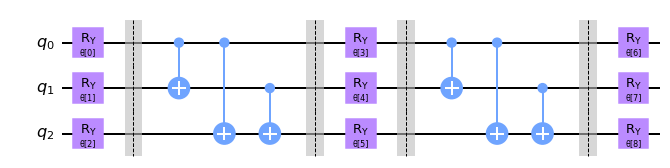
\includegraphics[width=\textwidth]{Artefact/Appendices/ansatz3-2.png}
    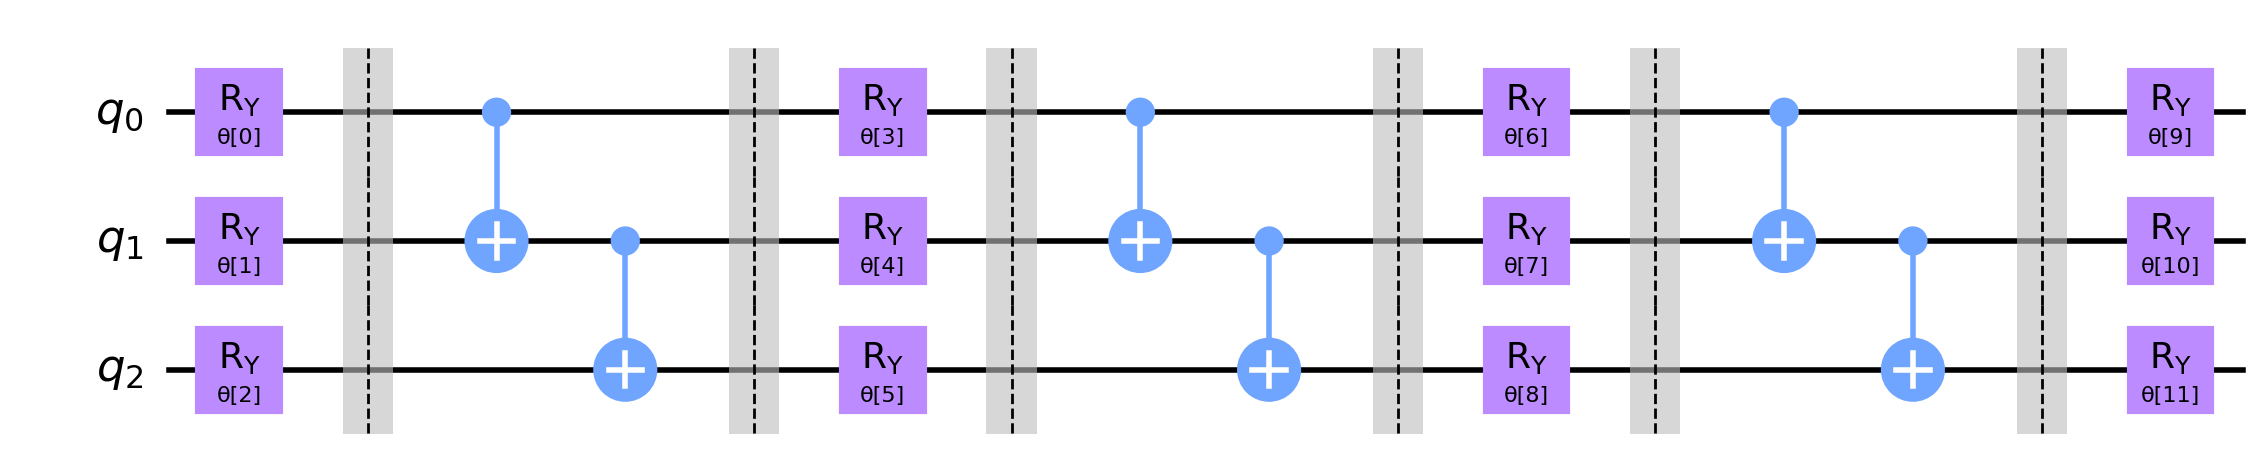
\includegraphics[width=\textwidth]{Artefact/Appendices/ansatz3-3.png}
    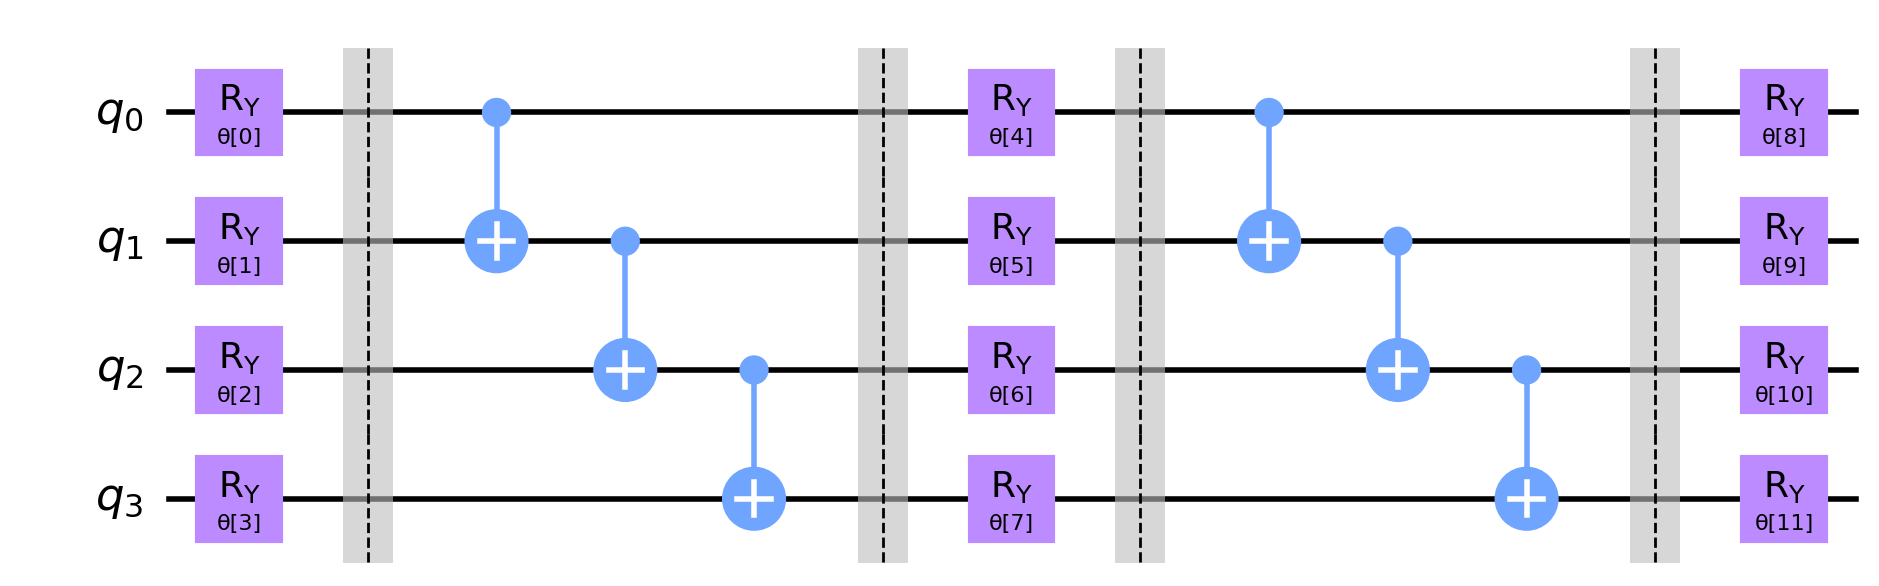
\includegraphics[width=\textwidth]{Artefact/Appendices/ansatz4-2.png}
    \caption{
        Samples of parameterised circuits generated by the Qiskit framework with 'full entanglement' option.
        The ansatz is a sequence of rotation layers and entanglement layers.
        Above: an ansatz of three qubits and two repetition layers.
        Middle: an ansatz of three qubits and three repetition layers.
        Below: an ansatz of four qubits and two repetition layers.
    }
    \label{Ansatz samples}
\end{figure}

\subsection{Treatments for ansatzes} \label{Sec: Treatments for ansatzes}
\todo{add method 2 and 3}
We apply the methods in Section \ref{Research Design section} to the ansatzes as described in section \ref{Sec: Creating Ansatzes}.

\subsubsection{Method \#0: Unrestricted} \label{Sec: Method0}
As discussed in the Section \ref{Research Design section}, the goal of this configuration is to produce a general multilayered perceptron network without any restriction.
The ansatzes will have unrestricted growth of circuit depth with a global cost function.
The initial parameters of this ansatz are randomised.
We implement the default ansatz to have the number of qubits and repetition increased iteratively.

\subsubsection{Method \#1: Local Cost Function and Shallow Depth Implementation} \label{Sec: Method1}
We implemented the \textit{Global Cost Function} as the measurement output for all qubits, while the \textit{Local Cost Function} is the measurement for the first two qubits.
Section \ref{Shallow Circuits, Local Cost Function section} and figure \ref{cost functions} previously explained the differences between the two cost functions.
The shallow ansatz is the same as the default.
However, the repetition number is kept as a constant number.

\subsubsection{Method \#2: Layerwise Learning} \label{Sec: Method2}
The ansatses will have unrestricted growth of circuit depth, and a measurement gate for each qubit at the end as the global cost function.
While the construction process is similar to that of the method \#0, we follow the \emph{Layerwise learning} algorithm as described in Section \ref{Sec: Layerwise Learning} to obtain the optimal initial parameters.

\subsubsection{Method \#3: Identity Blocks} \label{Sec: Method3}
For this method, we create a custom ansatz as an identity block.
As discussed in Section \ref{Sec: Identity blocks}, one identity block has two part, the first part can have its parameter randomised, while the second part invert the first part.
Figure \ref{Fig: Identity Ansatz Sample} demonstrate an identity block with two qubits.
For the first part of the identity block, we use the Real amplitudes with one repetition layer plus one rotation layer.
The gates of this part has their parameters randomised.
The second part of the identity block simply reverse the sequence of rotation layers and entanglement layers.
The gates of this part has their parameters chosen as invert of the first layer.
\begin{figure}
    \centering
    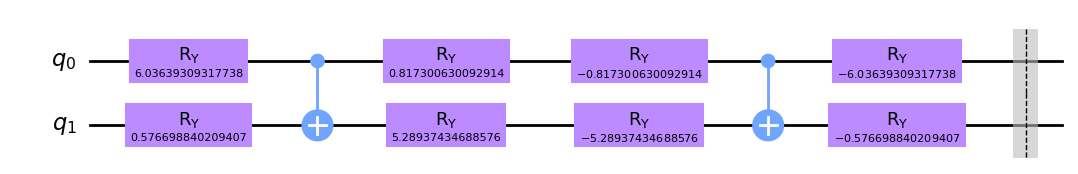
\includegraphics[width=\textwidth]{Artefact/Appendices/ansatz-identity.png}
    \caption{An Identity Block of two qubits, the first part has four random parameters, the second part is an invert of the first part.}
    \label{Fig: Identity Ansatz Sample}
\end{figure}


\subsection{Visualise the Variance} \label{Sec: Visualise the Variance}
\todo{move to design section}
We use the parameter shift rule from Eq. (\ref{Parameter-shift rules}) as implemented in the Qiskit Gradient library to calculate the gradient variance.
The BP phenomena can be verified when the gradient variance exponentially decreases with an increased number of qubits and repetition layers.

To visualise the gradient variances, we have plotted a range of random parameters for each ansatz as the initial starting point.
Such randomised parameters are generated 100 times uniformly to calculate the gradients.
We then plot the variance values of the gradients for different numbers of qubits and repetition values for a range of 2 to 7 qubits and ansatz layer repetition.
Note that the neural network generated in this experiment is not designed to answer a problem.
We will focus on the trainability of each method in the later phase of the experiment.

In short, we use 100 uniformly randomised parameters to scan the gradient.
Then we calculate the "slope" of the gradient.

\subsection{Classification Problem} \label{Sec: Classification Problem}
We implement a variational quantum classifier as previously discussed in the section \ref{VQA}.
The algorithm includes two stages: a training stage and a classification stage.
We use a dataset generated by Qiskit machine learning package for the algorithm.
The data was also used for a classification algorithm by Havlíček et al. \cite{havlicekSupervisedLearningQuantumenhanced2019}.

The quantum circuit for both stages is constructed from three parts: the feature map to encode data, the ansatz to perform optimisation and finally, a final rotation layer for measurement (see Figure \ref{Fig: Quantum circuit for classifier}).
The number of features will dictiate the number of qubits, in out case, we will be using two qubits for the quantum circuit.
For the method \#0 and \#2, there is no restriction on ansatz depth, so we build the ansatz to have 7 repetitions (15 depth units).
For the method \#1 with restriction for ansatz depth, we only use 2 reptitions (5 depth units).
For the customised ansatz in method \#3, we construct the ansatz to have the depth closer to that of method \#1 and \#2. We will be using three identity blocks as the ansatz, which results in 18 depth units.

The dataset consited of 50 labeled datapoints with two features is used for the traning stage.
The quantum circuit will be estimated as required by Gradient Descent algorithm provided by Qiskit to optimise the ansatz parameters.
For the classification satge, we use another set of 20 datapoints, and run the classifier with the optimised parameters obtained from the training stage.
The classifier would produce the predicted labels for each testing datapoint.
Then, we compare these predicted labels to the actual provided labels.

We collect the optimizer history (loss function per iteration) by implement a callback function for Gradient Descent algorithm.
The score $s$ of the classifier is calculate as the percentage likeliness of the predicted labels array compared to the actual labels array:
\begin{equation}
    s = 100\% (1 - \text{MSE})
\end{equation}
for $\text{MSE}$ is the mean square error of the actual labels array $Z$ and predicted labels array $\hat{Z}$ of length $n$:
\begin{equation}
    \text{MSE} = \frac{1}{n}\sum^n_{i=1}(Z_i - \hat{Z}_i)^2,
\end{equation}



\begin{figure}
    \centerline{
    \Qcircuit @C=1em @R=2em {
    \lstick{\ket{0}} & \multigate{1}{U_{\phi}(\vec{x})}    & \multigate{1}{W(\vec{\theta})}    & \meter & \rstick{z_1} \cw \\
    \lstick{\ket{0}} & \ghost{U_{\phi}(\vec{x})}           & \ghost{W(\vec{\theta})}           & \meter & \rstick{z_n} \cw \\
    }
    }
    \caption{
        Quantum Variational Classifier implemented for the experiment.
        The initial qubit state $\ket{0}^n$ is applied with a feature map $U_{\phi}(\vec{x})$ to encode data $\vec{x}$ from our dataset.
        Then, an unitary operation $W(\vec{\theta})$ is applied as the ansatz, follow up with a measurement layer.
        The output string $z \in \{0,1\}^n$ is mapped as label for the given datapoint $\vec{x}$.
    }
    \label{Fig: Quantum circuit for classifier}
\end{figure}


\subsection{Results and Analysis} \label{Result section}

\subsubsection{Sampling Gradients results}
\begin{table*}
    \centering
    \begin{tabular}{|| l l l ||}
        \hline
        \textbf{Ansatz} & \textbf{Method}                         & \textbf{Variance exponential fit} \\[0.5ex]
        \hline \hline
        Real Amplitude  & \#0: No restriction                     & -0.63                             \\
        Real Amplitude  & \#1: Local Cost function, shallow depth & -0.06                             \\
        Real Amplitude  & \#2: Layerwise Learning                 & -0.57                             \\
        Customised      & \#3: Identity Blocks                    & -0.60                             \\
        \hline
    \end{tabular}
    \caption{
        The phase one of the experiments that we implemented in the Python Notebook.
        We test the same ansatzes with different methods, we record the results as the vanishing rate of gradient when the number of qubits increased.
        The differences between the \emph{fit} values are small.
        However, consider the unit measure is \emph{exponential} (i.e. $10^{-1}, 10^{-2}$) the growth or decay rates can be significant.
    }
    \label{Tab: Experiment Phase 1 Res}
\end{table*}

Table \ref{Tab: Experiment Phase 1 Res} states all the combinations of ansatzes and methods.

The ansatz gradient variances decay as expected for the unrestricted setting.
The decay rate is exponentially fitted with the rate of -0.63.
The figure \ref{Plot ansatzes variance}a shows the results of the ansatz in this configuration.
The semi-log plots portray the variances of gradient from the ansatz in the unrestricted configuration.
Consider that the unit measure for variance is in \emph{exponential} form, so the linear graph is exponentially closer to zero for each qubit added to the circuit.
This result indicates that the cost function landscape becomes flatter and flatter.
Eventually, the gradient would reach a near-zero value across a large plateau, which would be inefficient for any gradient-based optimization algorithm to train the model.
We discussed this phenomenon in Section \ref{Barren Plateaus section}.

\todo{changing the number to actual name}
\begin{figure}
    \centering
    \begin{subfigure}[b]{.49\linewidth}
        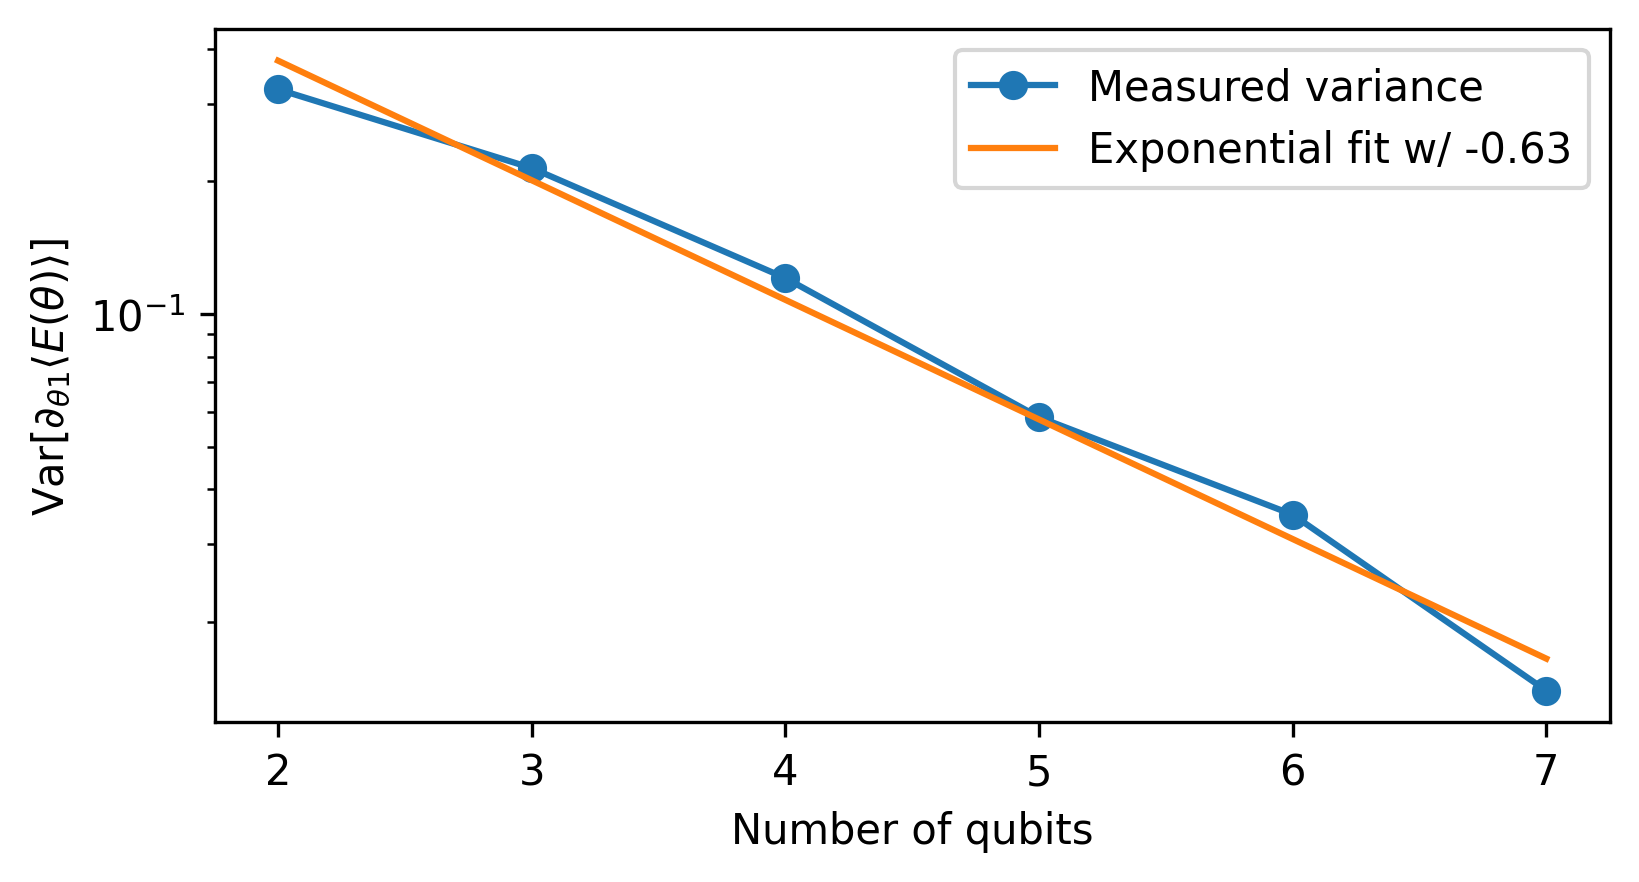
\includegraphics[width=\linewidth]{Artefact/Appendices/var0.png}
        \centerline{0) Default method}
    \end{subfigure}
    \hfill
    \begin{subfigure}[b]{.49\linewidth}
        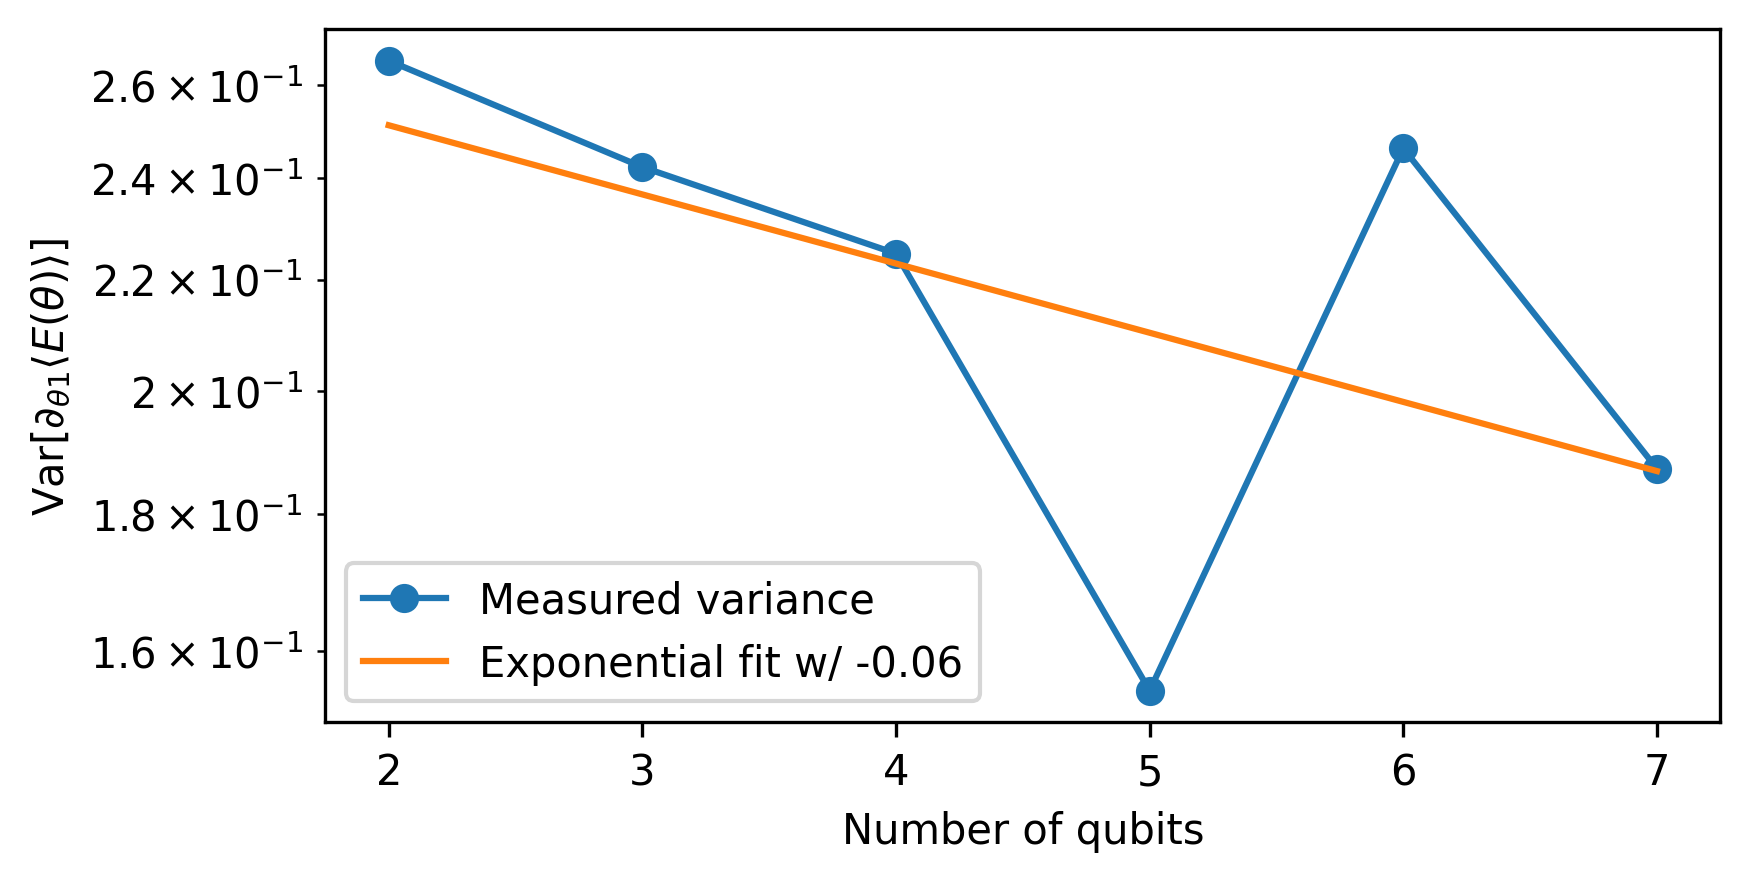
\includegraphics[width=\linewidth]{Artefact/Appendices/var1.png}
        \centerline{1) Shallow circuit and local cost function}
    \end{subfigure}

    \begin{subfigure}[b]{.49\linewidth}
        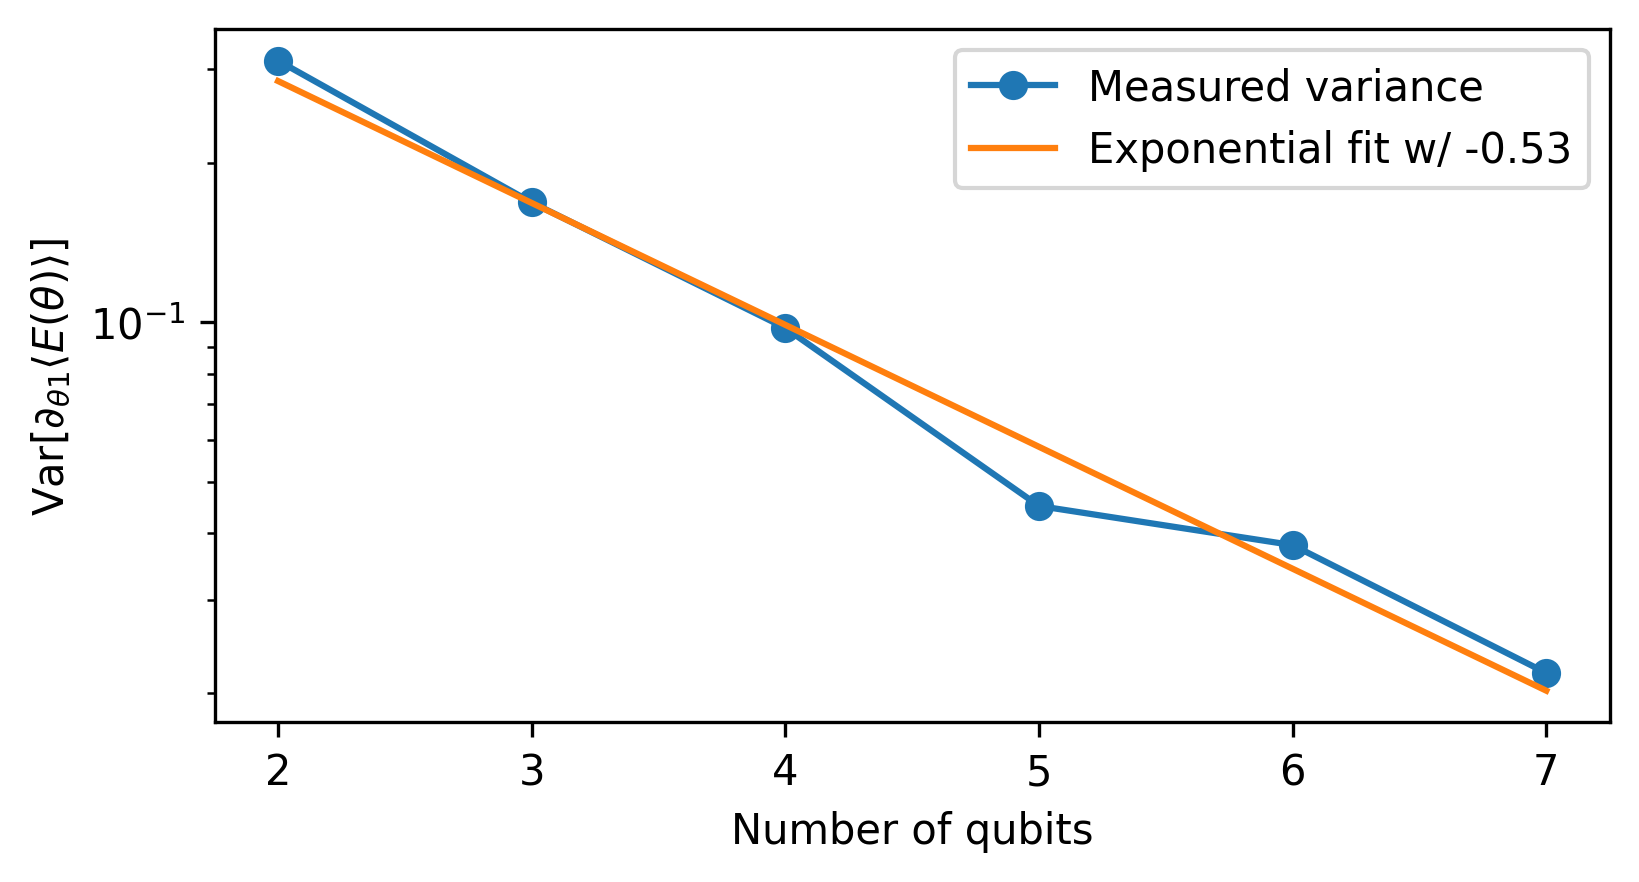
\includegraphics[width=\linewidth]{Artefact/Appendices/var2.png}
        \centerline{2) Layerwise learning}
    \end{subfigure}
    \hfill
    \begin{subfigure}[b]{.49\linewidth}
        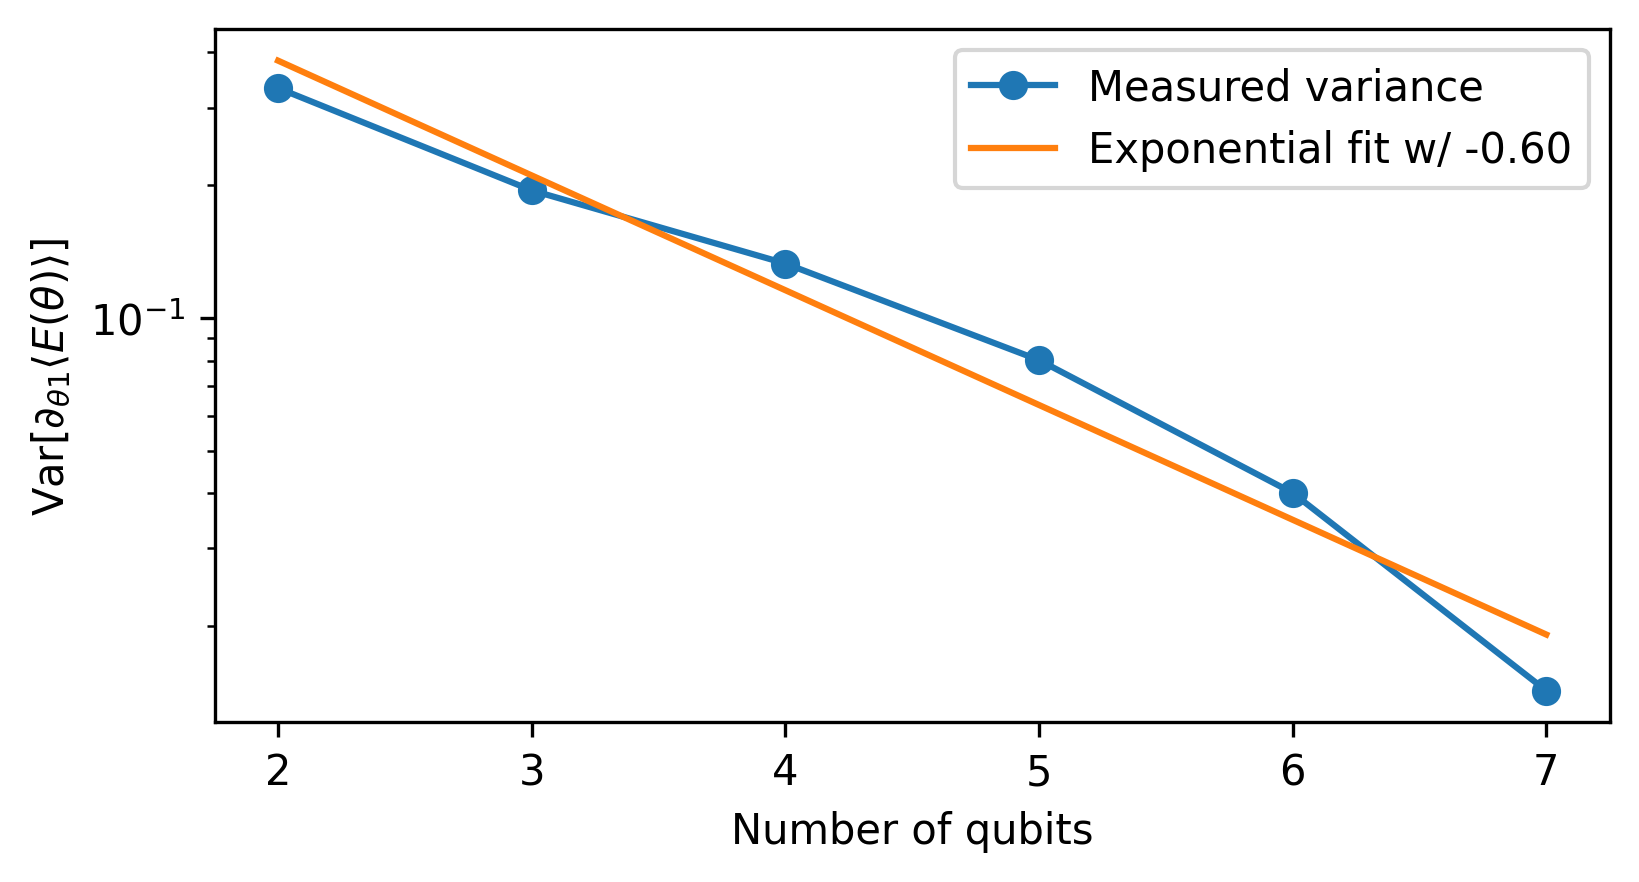
\includegraphics[width=\linewidth]{Artefact/Appendices/var3.png}
        \centerline{3) Identity blocks}
    \end{subfigure}

    \caption{
        The variances of gradient from differences ansatzes in the four configurations.
        For each iteration, we increase the qubit and repetition count by 1, starting from 2 to 7.
        The variances vanish exponentially to the number of qubits.
        For the shallow circuit - local cost function, we keep the repetition value fixed as 1 and only measure two qubits.
    }
    \label{Plot ansatzes variance}
\end{figure}

In contrast, for the case of Local Cost Function and Shallow circuit, we observe that the variances of the ansatz' gradient did not vanish when we attempted to increase the number of qubits.
The slope of the ansatz in this case decay exponentially fit with -0.06.
This implies that the cost function landscape can sustain the slope.
Figure \ref{Plot ansatzes variance}b shows the result of the experiment for local cost function and shallow circuit.
We can see that the ansatz produced an unstable graph which mean the trainability of gradient-based optimization algorithms would not be consistent.
For example, the variance value for 6 qubits is higher compared to 3, 4 or 5 qubits.

To compare the effectiveness of the different treatments, we plot the variance graph of above mention cases in Figure \ref{Fig: Plot Variances} and the Table \ref{Tab: Experiment Phase 1 Res}.
The results have shown the differences in the decay rates of different ansatzes and methods.
Overall, the ansatzes with the local cost function and restriction on circuit depth have their variance values remaining higher and being more consistent for higher qubit count.
The ansatz with this treatment, therefore would not possess a barren plateau.
On the other hand, the values for the other cases shrink exponentially and eventually, the near-zero gradient around the initial point will expand to a large plateau.


\begin{figure}
    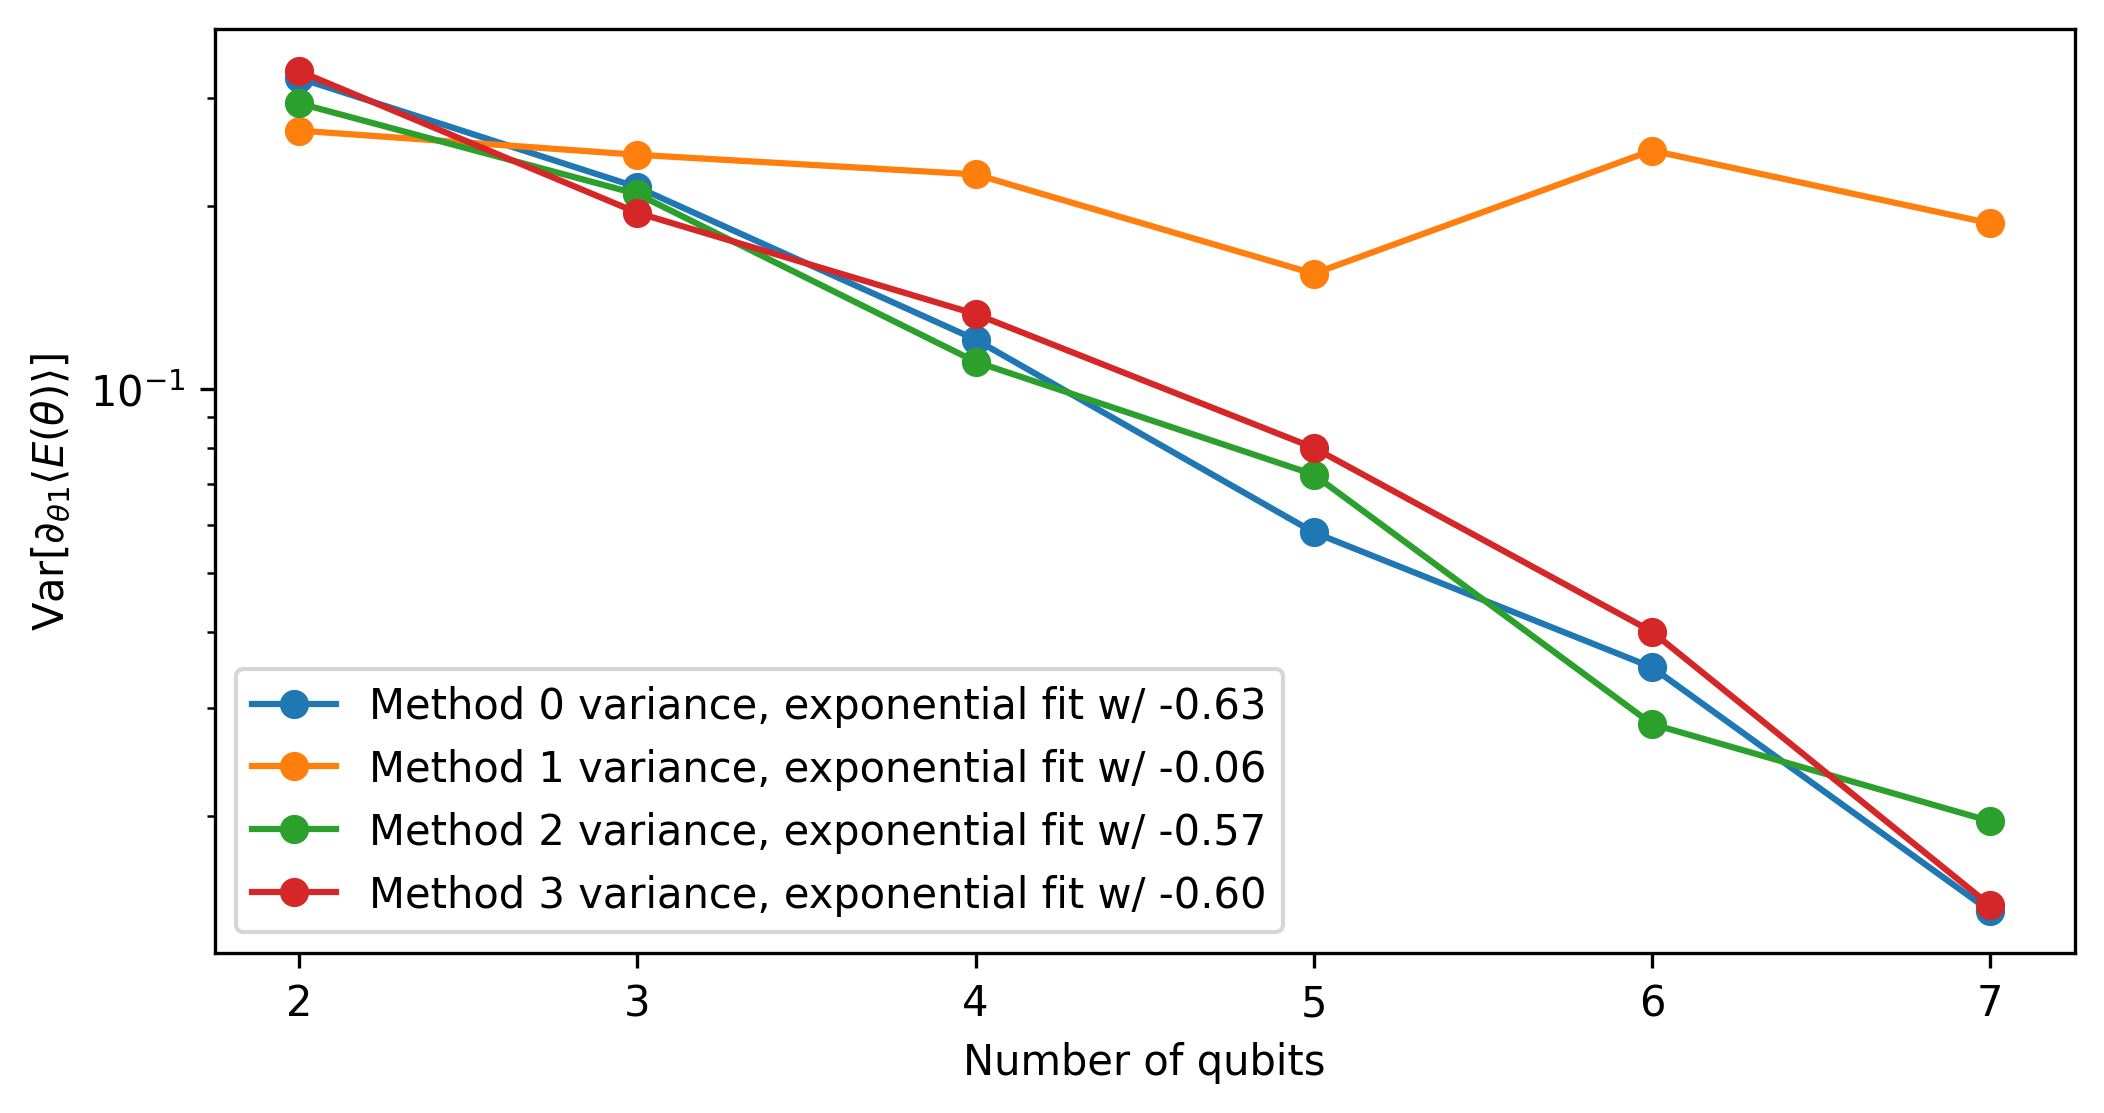
\includegraphics[width=\linewidth]{Artefact/Appendices/variances.png}
    \caption{
        Comparison of the variance values of the ansatzes with four treatments applies.
        The ansatz with local cost function and fixed depth has its variance decay at a significantly smaller rate (-0.06) compared to the rest.
    }
    \label{Fig: Plot Variances}
\end{figure}


\subsubsection{Classification Results}

\begin{table*}
    \centering
    \begin{tabular}{|| p{4cm} p{2cm} p{2cm} p{2cm} p{2cm} ||}
        \hline
        \textbf{Method}                          & \textbf{Circuit depth} & \textbf{Parameters count} & \textbf{Minimum loss} & \textbf{Score} \\
        \hline \hline
        0: No Restriction                        & 15                     & 16                        & 0.57                  & 72.50\%        \\
        1: Local Cost Function - Shallow circuit & 5                      & 6                         & 0.57                  & 80\%           \\
        2: Layerwise Learning                    & 15                     & 16                        & 0.39                  & 92.5\%         \\
        3: Identity Blocks                       & 18                     & 24                        & 0.39                  & 90\%           \\
        \hline
    \end{tabular}
    \caption{
        The result as recorded from the phase two of the experiment.
        We use the ansatzes from four methods as the neural network to solve a classification problem.
    }
    \label{Tab: Experiment Phase 2 Res}
\end{table*}

The unrestricted and local cost function - shallow depth ansatzes loss functions both converged at a value of 0.57.
However, we can see that the local cost function and shallow circuit ansatz achieved higher accuracy in the classification test (at 80\% accuracy) than the unrestricted ansatz (at 72.5\% accuracy).
However, by restricting the ansatz depth, we may have limited the model capacity, this also applies to classical machine learning \cite{ianDeepLearningAdaptive2016}.
As more complex functions would require higher model capacity, thus higher layer count and qubit count, the local cost function - shallow depth method is suitable if the dataset represents a simple function.

\todo{) may have BP, but 1 does not have cap enough to learn, so it converged but still very high}

The identity blocks can achieve a similar loss value as the layerwise learning method (0.39) with a bit lower accuracy.
We can see that with the optimised initial parameters, the loss function can converge faster compared to identity blocks initialisation.
However, it would take more time to obtain the optimal initial parameter due to the training process (see Section \ref{Sec: Method2}), while it is much faster to generate parameters for identity blocks in Section \ref{Sec: Method3}.
The two methods also have their accuracy close to each other, scoring at 92\% for layerwise learning and 90\% for identity blocks.
Thus they are suitable for designing ansatzes of higher layer count to learn more complex functions.


To compare the effectiveness of different approaches, we plot the loss per iteration graph of above mention cases in Figure \ref{Fig: Plot Loss and Accuracy} and Table \ref{Tab: Experiment Phase 2 Res}
Overall, the methods that involve configurations on the initial parameters can achieve lower loss in training and higher score on the classification test.

\begin{figure}
    \begin{subfigure}{\linewidth}
        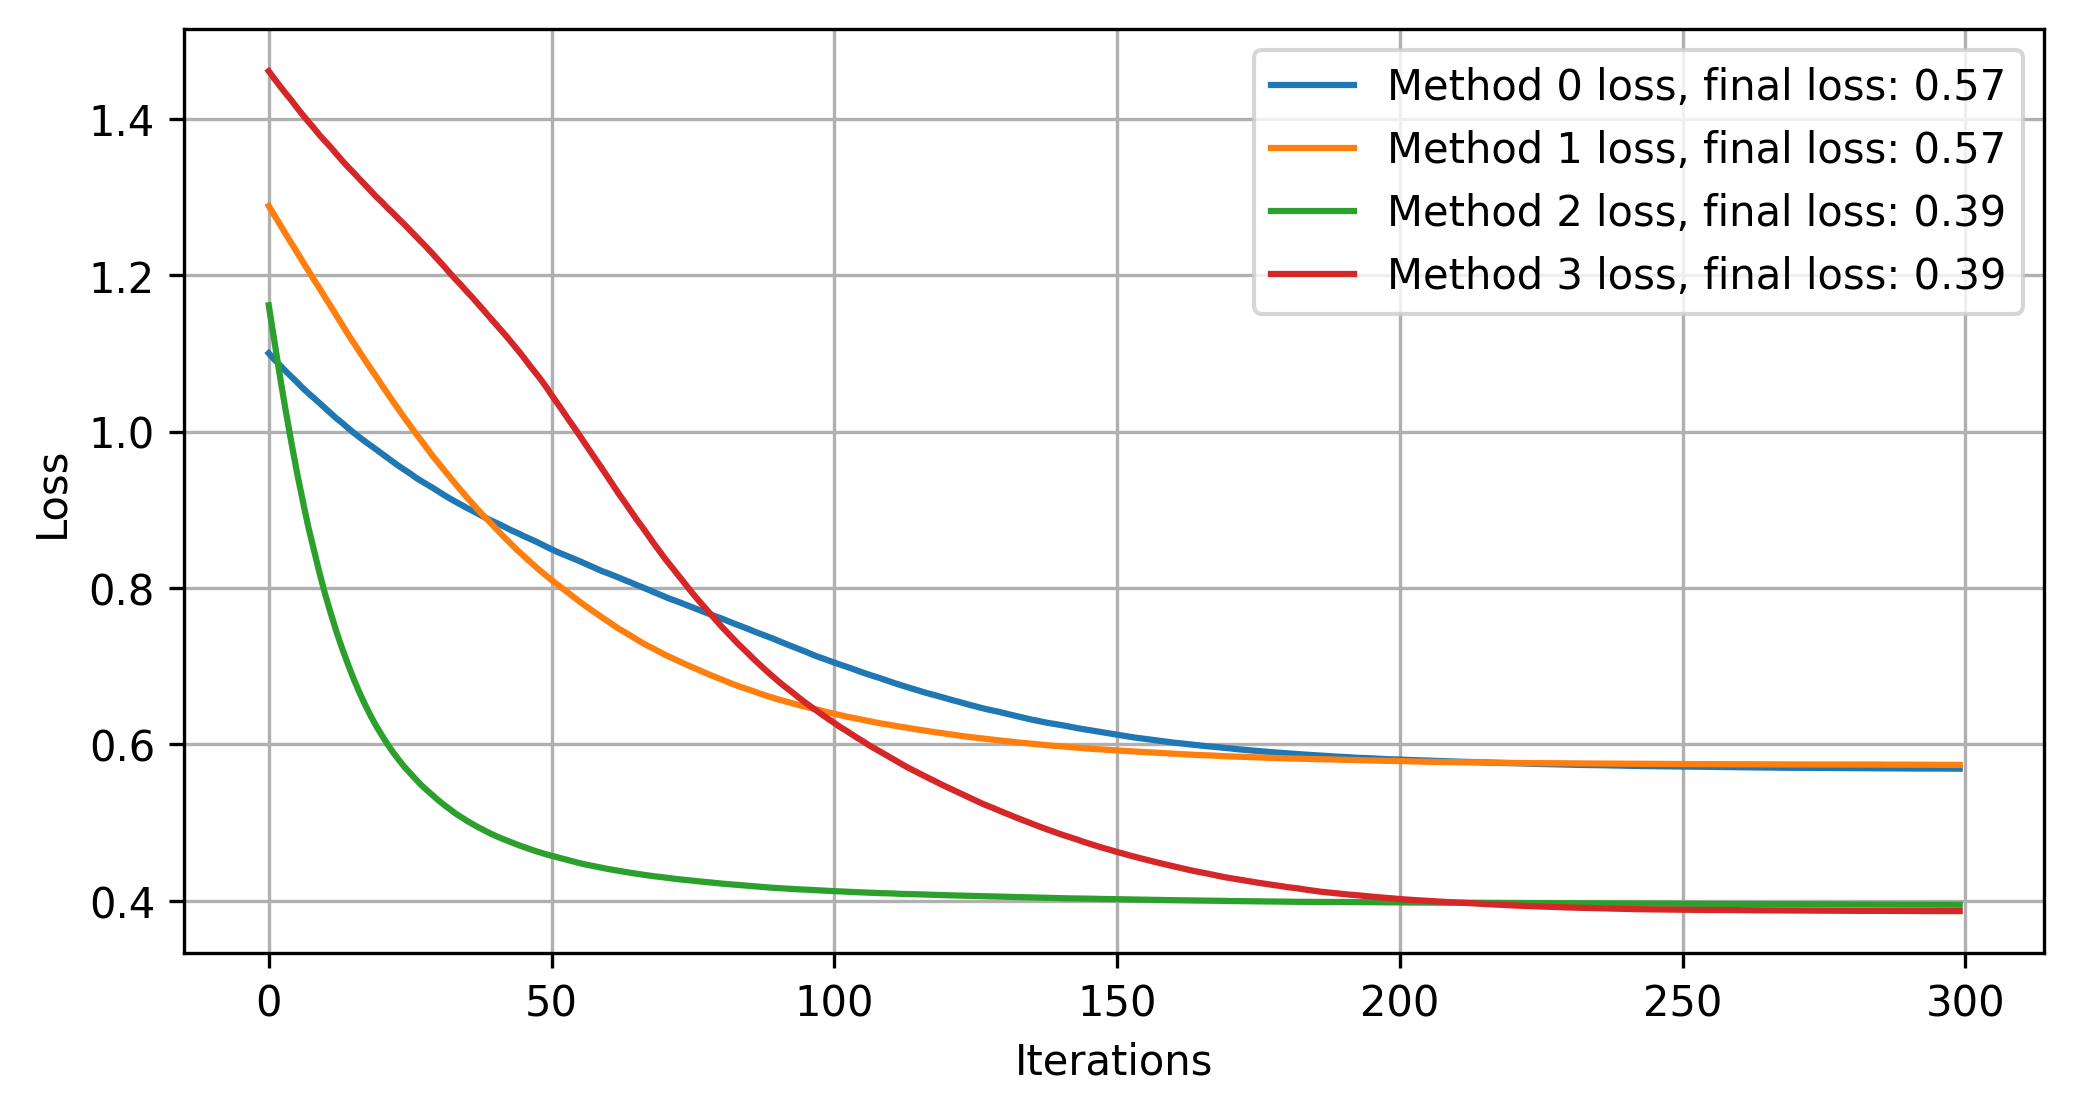
\includegraphics[width=\linewidth]{Artefact/Appendices/loss.png}
        \centerline{a) Loss function values of four classifiers in 300 steps}
    \end{subfigure}
    \begin{subfigure}{\linewidth}
        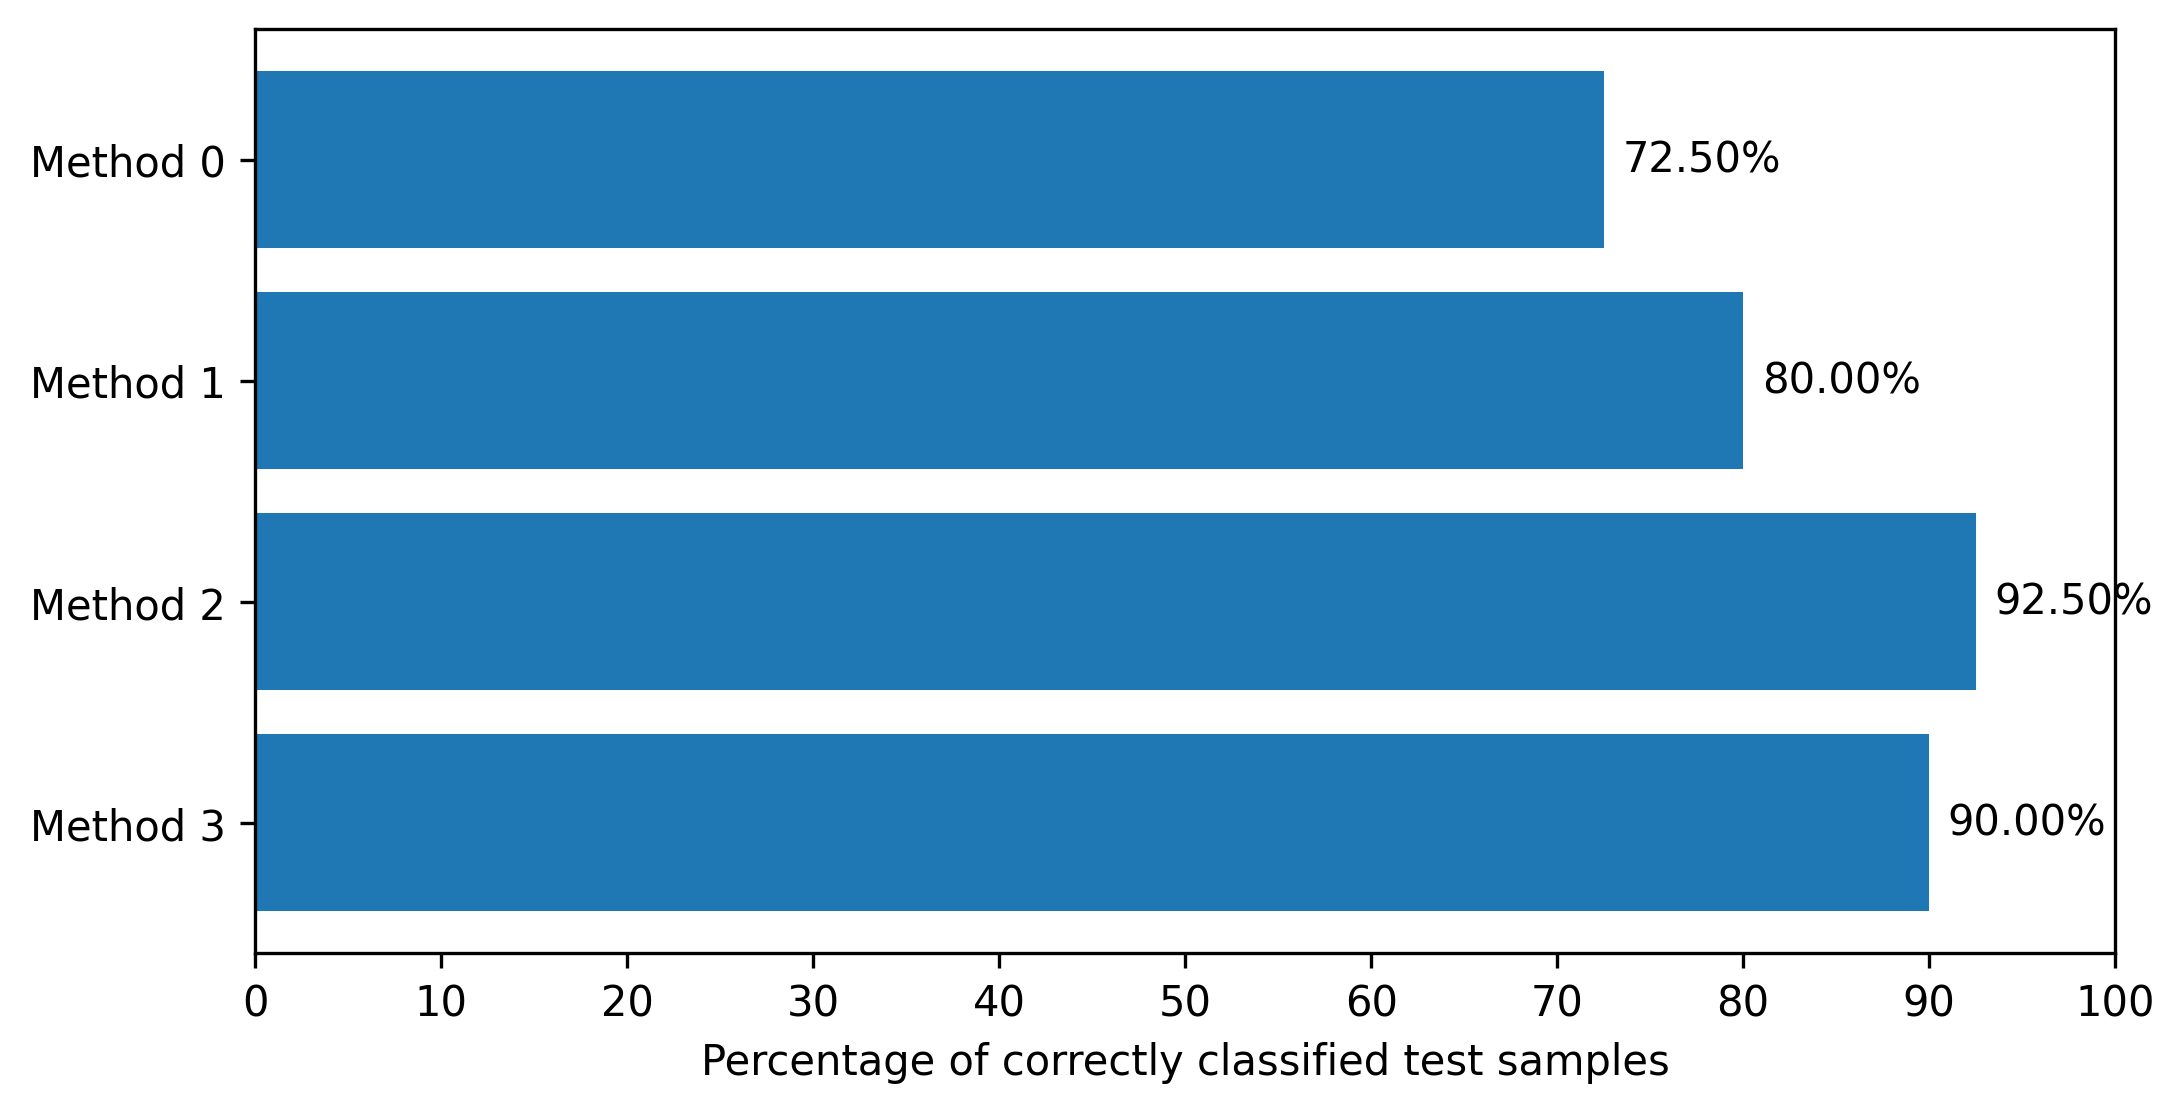
\includegraphics[width=\linewidth]{Artefact/Appendices/accuracy.png}
        \centerline{b) Accuracy score of four classifiers}
    \end{subfigure}

    \caption{
        Comparison of the loss values per iteration of gradient descent for the ansatzes with four treatments applies.
        We measure the accuracy of prediction with a set of 20 testing datapoints.
    }
    \label{Fig: Plot Loss and Accuracy}
\end{figure}


\subsection{Artefact Development Summary}

We have implemented three methods of dealing with barren plateau by altering the ansatz's depth, cost function, and initial parameters aspects.
The experiments have produced the results as the slopes of the gradients for a number of qubits, as well as the performance of ansatzes in neural network training.
The results indicate that the variances of the gradient can be stable if we set a limit on the length of the circuit and the cost function, and the training performance can increase if we carefully select the initial parameters.

With this artefact, we have addressed the research design in Section \ref{Research Design section}.
We have implemented the three methods, namely \textit{local cost function, shallow ansatz depth}, \textit{layerwise learning} and \textit{identity blocks}.
We have compared the variances in the first phase of the experiment.
We anticipate that a higher variance value does not mean the optimisation is going in the right direction, the model can still stick it in a local minimum, or the error landscape is random.
To verify the performance of these methods, in the second phase, we implemented a variational quantum neural network to solve a classification problem with a standard dataset.

The phase two of the experiments have verified that the unrestricted configuration may have run into a barren plateau, while the others can converge to their minimums - the answers.
Moreover, these experiments are conducted in an emulated environment with a noise model from \emph{ibm\_perth} backend.
Thus, this experiment can reflect the real-life situation to some extent.

According to Figure \ref{Fig: Plot Variances}, the variance values of the limited depth - cost function method at seven qubits configuration is significantly higher than the rest.
At higher qubit configuration, the barren plateaus are also more likely to appear, and the performance of these methods under this phenomenon is worth investigating.


    \bibliographystyle{jcabbrv} % Sorted and "note" fields removed
\bibliography{src/References/zoteroReferences.bib}
\end{document}
